\documentclass[review,12pt]{elsarticle}

\usepackage{hyperref}
\usepackage{amsmath,amssymb,amsfonts,amsthm}
\usepackage{booktabs}
\usepackage{tabularx}
\usepackage{threeparttable}
\usepackage{array}
\usepackage{geometry}
\usepackage{graphicx}
\usepackage{pgfplots}
\usepackage{pgfplotstable}
\usepackage{tikz}
\usepackage{float}
\usepackage{caption}
\usepackage{subcaption}
\usepackage{natbib}
\usepackage{xcolor}
\usepackage{enumitem}
\usepackage{url}
\usepackage{microtype}

\pgfplotsset{compat=1.18}
\usepgfplotslibrary{fillbetween}
\geometry{a4paper, margin=1in}
\raggedbottom

% ── Caption Spacing & Custom Column Definitions ───────────────
\captionsetup[table]{skip=6pt}
\captionsetup[figure]{skip=6pt}

\newcolumntype{Y}{>{\centering\arraybackslash}X}
\newcolumntype{L}{>{\raggedright\arraybackslash}X}
\newcolumntype{R}{>{\raggedleft\arraybackslash}X}
\newcolumntype{C}[1]{>{\centering\arraybackslash}p{#1}}

\journal{The Journal of Economic Asymmetries}

\newtheorem{theorem}{Theorem}
\newtheorem{lemma}{Lemma}
\newtheorem{corollary}{Corollary}
\newtheorem{proposition}{Proposition}
\newtheorem{hypothesis}{Hypothesis}

\begin{document}

\begin{frontmatter}

\title{Asymmetric Cost-Channel Monetary Transmission and Policy-Rate Thresholds: Evidence from Egypt}

\author[idsc,cu]{Mohamed Fawzy AbdulAziz\corref{cor1}}
\ead{mohamed.abdulaziz@idsc.gov.eg}

\cortext[cor1]{Corresponding Author: Research Department, Information and
Decision Support Center (IDSC), The Egyptian Cabinet, 1 Magles El Shaab St.,
Cairo, Egypt. Affiliated with the Department of Economics, Faculty of Economics
and Political Science, Cairo University, Giza, Egypt.}

\address[idsc]{Information and Decision Support Center (IDSC), The Egyptian Cabinet, Cairo, Egypt}
\address[cu]{Department of Economics, Faculty of Economics and Political Science, Cairo University, Giza, Egypt}

\begin{abstract}
Standard New Keynesian Phillips Curve (NKPC) formulations assume symmetric
price-setting frictions and treat nominal interest rate adjustments exclusively
as aggregate demand shifters. In import-dependent emerging economies with
working-capital credit dependence, however, monetary tightening simultaneously
acts as a direct marginal cost shock, generating dynamics consistent with the empirical
``Price Puzzle''. This paper makes four contributions to monetary economics.
First, we develop a micro-founded derivation of the \textit{Hybrid Asymmetric Cost-Channel
New Keynesian Phillips Curve} (ACC-NKPC). By integrating firm-level idiosyncratic cost
shocks $\nu_{jt} \sim \mathcal{N}(0,\sigma_\nu^2)$, endogenous probability measure aggregation
$\omega_t = \Phi(\Delta MC_t / \sigma_\nu)$, backward-looking price indexation ($\gamma$),
and working-capital borrowing constraints ($\chi$), we micro-found state-dependent
Calvo pricing ($\theta^+ \neq \theta^-$). Second, we derive the \textit{Threshold Inversion
Proposition} ($\phi^+ > \kappa/\sigma$) establishing the structural condition under which the
cost channel dominates the aggregate demand channel. Using the \citet{hansen2000} threshold
framework with lagged policy rates ($i_{t-1}$) to mitigate contemporaneous simultaneity across
the empirical $10\%$--$90\%$ distribution support, we identify an empirical switching point of
$i^* = 20.0\%$ (Hansen likelihood-ratio 95\% confidence set: $[18.5\%,\;21.5\%]$). Conditional
on macroeconomic calibration, implied Calvo stickiness is $\theta^+ = 0.548$ ($2.2$ months)
for upward adjustments versus $\theta^- = 0.832$ ($6.0$ months) for downward adjustments,
consistent with a ``Rockets and Feathers'' pricing pattern. Third, structural Two-Step Optimal
GMM and HAC-OLS estimates on monthly Egyptian data spanning $2011\text{M}01$--$2026\text{M}04$ ($T=184$)
show that interest rate hikes transmit positively to inflation below the threshold
($\phi_{\text{Low}}^{+} = 1.8783,\; p < 0.001$), while exchange rate pass-through is strongly
asymmetric ($\lambda^{+} = 8.2912,\; p = 0.002$). Results are robust across a set of theory-motivated
external instruments with documented relevance and sensitivity to alternative exclusion sets
(omitting oil prices, IMF dummies, and spread proxies; Kleibergen--Paap $F = 28.4$,
Hansen $J$ $p = 0.512$), alternative \citet{hamilton2018} activity gap proxies, polynomial
specifications, linear splines, and full Nonlinear ARDL (NARDL) error correction models
($\text{ECT}_{t-1} = -0.3210^{***}, \text{Bounds } F = 7.82, p < 0.01$). Fourth, machine learning
models (Gradient Boosting, Random Forest, SVR) provide complementary predictive validation
($\text{RMSE}=3.060\text{ pp}$; Diebold--Mariano $p < 0.001$), with SHAP and partial dependence
functions recovering a qualitatively similar non-linear dependence around $19.8\%$--$20.0\%$
trained exclusively on raw macroeconomic observables. Multi-year policy fan charts and conditional
scenario matrices are documented.
\end{abstract}

\begin{keyword}
Asymmetric Cost Channel \sep New Keynesian Phillips Curve \sep Price Puzzle
\sep Working Capital Frictions \sep Exchange Rate Pass-Through \sep Threshold
Econometrics \sep Machine Learning \sep Egypt
\JEL E31 \sep E52 \sep F31 \sep C22 \sep C45 \sep C53 \sep O11
\end{keyword}

\end{frontmatter}

% ══════════════════════════════════════════════════════════════
\section{Introduction}
\label{sec:intro}
% ══════════════════════════════════════════════════════════════

The transmission mechanism of monetary policy to consumer price inflation is a
central pillar of macroeconomic theory. In the canonical New Keynesian framework
\citep{clarida1999, woodford2003, gali2008}, nominal interest rate adjustments operate
primarily through the \textit{aggregate demand channel}: an increase in the policy
rate raises real borrowing costs, depresses consumption and investment, induces a
negative output gap ($\tilde{y}_t < 0$), and gradually lowers inflation.

However, in credit-constrained, import-dependent emerging market economies, central
banks frequently encounter an empirical phenomenon where interest rate hikes are
followed in the short run by an acceleration of headline inflation. This phenomenon---conventionally termed the ``Price Puzzle''---has historically been attributed to omitted forward-looking information in central bank reaction functions \citep{sims1992, bernanke1998}. Under the \citet{sims1992} signaling hypothesis, if policymakers anticipate future inflation and tighten preemptively, standard VAR models without adequate expectation proxies spuriously attribute rising inflation to the preceding rate hike. By explicitly incorporating model-consistent forward-looking inflation expectations ($\mathbb{E}_t[\pi_{t+1}]$) and global commodity supply controls ($\text{OIL}_t$), our structural GMM specification directly rules out the Sims omitted-variable critique. Instead, the persistent positive response is micro-founded in the \textit{Cost Channel of Monetary Policy} \citep{barth2001, ravenna2006, chowdhury2006}:
when domestic enterprises rely on short-term commercial bank credit to finance working-capital
outlays (wages and imported intermediate materials) prior to sales realisation, nominal
interest rates directly enter the firm's marginal cost schedule. Under substantial working-capital
dependence, policy rate increases act as adverse cost-push shocks that elevate prices in the short run.

Despite extensive inquiries into cost-channel dynamics \citep{tillmann2008, hulsewig2009},
the existing literature exhibits two major limitations:

\begin{enumerate}[label=\textbf{(\arabic*)}]
\item \textbf{The Symmetry Assumption.} Canonical NKPC formulations uniformly impose
symmetric Calvo pricing ($\theta^{+} = \theta^{-}$) and linear interest-rate pass-through.
In emerging economies characterized by imperfect competition and foreign exchange illiquidity,
firms face asymmetric survival incentives: cost increases are passed forward rapidly to protect
operating margins, whereas cost reductions are retained to rebuild retained earnings
\citep{peltzman2000, shin2014, brun2017, delatte2012}.

\item \textbf{Absence of Endogenous Policy Thresholds.} The relative strength of the
cost channel versus the aggregate demand channel is unlikely to be invariant across all
interest rate environments. At moderate policy rates, working-capital cost pressures can
dominate; at elevated rates, credit contraction and debt service burdens severely compress
aggregate demand, re-establishing conventional disinflationary transmission. Identifying
this switching point requires formal threshold econometrics \citep{hansen2000}.
\end{enumerate}

This study addresses these gaps by developing a micro-founded \textit{Hybrid Asymmetric
Cost-Channel NKPC} (ACC-NKPC) and empirically testing it on monthly Egyptian data over
the period $2011\text{M}01$--$2026\text{M}04$ ($T=184$). Egypt provides an exceptional empirical
setting: between 2016 and 2026, the Central Bank of Egypt (CBE) navigated multiple foreign
exchange floatation waves and raised its policy rate by over 1,800 basis points (reaching
$27.25\%$ in 2024 before gradual normalization).

The study makes four contributions:
\begin{enumerate}[label=\textbf{(\roman*)}]
\item \textbf{Micro-Foundations with Idiosyncratic Shocks:} We derive the ACC-NKPC
from first principles, introducing idiosyncratic cost shocks $\nu_{jt} \sim \mathcal{N}(0,\sigma_\nu^2)$
to provide an explicit probability-measure aggregation $\omega_t = \Phi(\Delta MC_t / \sigma_\nu)$,
along with backward-looking price indexation ($\gamma$) that bridges forward-looking expectations
and empirical inflation persistence.
\item \textbf{Threshold Inversion Proposition:} We formally derive the mathematical
condition under which the cost channel dominates ($\phi^+ > \kappa/\sigma$) and identify
the empirical threshold at $i^* = 20.0\%$ using \citet{hansen2000} threshold methods
with lagged policy rates ($i_{t-1}$) to mitigate contemporaneous simultaneity.
\item \textbf{Robust Econometric Identification:} We estimate the structural equation
via Two-Step Optimal GMM and HAC-OLS, utilizing theory-motivated external instruments
(US Federal Funds rate, global commodity prices, banking spreads, IMF dummies; Kleibergen--Paap
$F = 28.4$, Hansen $J$ $p = 0.512$), and confirm robustness across \citet{hamilton2018} output
gap proxies, polynomial specifications, linear splines, and full Nonlinear ARDL (NARDL) models.
\item \textbf{Machine Learning Predictive Validation:} We show that tuned tree-based
ensembles (GBM, Random Forest) achieve superior out-of-sample forecasting accuracy
($\text{RMSE}=3.060\text{ pp}$) and recover a qualitatively similar non-linear dependence
around $19.8\%$--$20.0\%$ via SHAP and partial dependence analysis on raw macro features.
\end{enumerate}

The remainder of this paper is structured as follows. Section~\ref{sec:theory}
presents the theoretical model. Section~\ref{sec:data} describes the data and
pre-estimation diagnostics. Section~\ref{sec:empirical} presents the structural
econometric results. Section~\ref{sec:ml} provides machine learning benchmarking
and threshold analysis. Section~\ref{sec:policy} discusses policy implications
and conditional scenario projections. Section~\ref{sec:conclusion} concludes.

% ══════════════════════════════════════════════════════════════
\section{Theoretical Framework: The Micro-Founded Hybrid ACC-NKPC}
\label{sec:theory}
% ══════════════════════════════════════════════════════════════

\subsection{Household Sector and Aggregate Demand}

The economy is populated by a continuum of identical, infinitely lived households
maximising expected discounted intertemporal utility:
\begin{equation}
\max_{\{C_t,L_t,B_t\}} \mathbb{E}_0 \sum_{t=0}^{\infty} \beta^t
\left[\frac{C_t^{1-\sigma}}{1-\sigma} - \frac{L_t^{1+\varphi}}{1+\varphi}\right]
\label{eq:utility}
\end{equation}
subject to the nominal budget constraint:
\begin{equation}
P_t C_t + \frac{B_t}{1+i_t} \le B_{t-1} + W_t L_t + \Pi_t + T_t
\label{eq:budget}
\end{equation}
where $\beta \in (0,1)$ is the subjective discount factor, $\sigma > 0$ is the
inverse intertemporal elasticity of substitution, $\varphi > 0$ is the inverse
Frisch labour supply elasticity, $C_t$ is consumption, $L_t$ is labour supply,
$B_t$ is nominal bond holdings, $W_t$ is the nominal wage, and $\Pi_t$ denotes
firm profits. The first-order conditions yield the standard Euler equation:
\begin{equation}
\beta (1+i_t) \mathbb{E}_t \left[\left(\frac{C_{t+1}}{C_t}\right)^{-\sigma} \frac{P_t}{P_{t+1}}\right] = 1
\label{eq:euler}
\end{equation}
Log-linearising \eqref{eq:euler} around the steady state yields the Dynamic IS curve:
\begin{equation}
\tilde{y}_t = \mathbb{E}_t[\tilde{y}_{t+1}] - \frac{1}{\sigma}(i_t - \mathbb{E}_t[\pi_{t+1}] - r_t^n)
\label{eq:is}
\end{equation}
where $\tilde{y}_t \equiv y_t - y_t^n$ is the output gap and $r_t^n$ is the natural real interest rate.

\subsection{Firms, Working Capital, and Idiosyncratic Cost Shocks}
\label{sec:firm}

A continuum of monopolistically competitive intermediate goods producers $j \in [0,1]$
produce differentiated goods via Cobb-Douglas technology:
\begin{equation}
Y_t(j) = A_t L_t(j)^{1-\alpha} M_t(j)^{\alpha}, \qquad \alpha \in (0,1)
\label{eq:prod}
\end{equation}
where $A_t$ is total factor productivity, $L_t(j)$ is domestic labour, and $M_t(j)$
represents imported intermediate materials.

\textbf{Working-Capital Financing.} Intermediate firms must finance a fraction
$\chi \in [0,1]$ of their total nominal production costs in advance via short-term
commercial bank credit at the corporate lending rate $i_t^L = i_t + \text{Spread}_t$,
where $i_t$ is the CBE nominal policy rate and $\text{Spread}_t \equiv \mu_t^b$ is the
commercial banking spread reflecting financial intermediation costs and credit risk.
Total nominal production costs for firm $j$ are:
\begin{equation}
TC_t(j) = \bigl[W_t L_t(j) + E_t P_t^{*} M_t(j)\bigr](1 + \chi i_t^L) \exp(\nu_{jt})
\label{eq:cost}
\end{equation}
where $E_t$ is the nominal exchange rate (EGP/USD), $P_t^{*}$ is the foreign price
of imported inputs, and $\nu_{jt} \sim \text{i.i.d. } \mathcal{N}(0, \sigma_\nu^2)$
represents firm-specific idiosyncratic productivity/cost shocks.

Minimising \eqref{eq:cost} subject to \eqref{eq:prod} yields the aggregate nominal
marginal cost:
\begin{equation}
MC_t = \frac{1}{A_t}\left(\frac{W_t}{1-\alpha}\right)^{1-\alpha}\left(\frac{E_t P_t^{*}}{\alpha}\right)^{\alpha}(1 + \chi i_t^L)
\label{eq:mc}
\end{equation}
Log-linearising around the steady state $(i_{ss}, E_{ss}, A_{ss})$ yields:
\begin{equation}
\widehat{mc}_t = (\sigma+\varphi)\tilde{y}_t + \alpha \hat{e}_t + \tilde{\mu} \tilde{i}_t + u_t
\label{eq:mc_linear}
\end{equation}
where $\tilde{\mu} \equiv \frac{\chi}{1 + \chi i_{ss}}$ is the structural working-capital intensity. In open emerging economies with foreign-currency external liabilities, commercial banking spreads and corporate risk premia directly reflect sovereign foreign exchange liquidity and reserve adequacy \citep{shin2014}:
\begin{equation}
\widehat{\text{Spread}}_t = -\eta_b \text{Buff}_t + \varepsilon_t^b, \qquad \text{Buff}_t \equiv \ln\left(\frac{\text{FX\_RES}_t}{\overline{\text{FX\_RES}}}\right)
\label{eq:spread_buffer}
\end{equation}
where $\text{Buff}_t$ captures deviations of gross official foreign reserves from their historical sample mean. Substituting \eqref{eq:spread_buffer} into the marginal cost disturbance yields the composite aggregate pricing term $\eta \cdot \text{Buff}_t$ in \eqref{eq:acc_nkpc} with theoretical slope $\eta = -\tilde{\mu}\eta_b < 0$, while the orthogonalized disturbance $u_t \equiv -\hat{a}_t + \tilde{\mu}\varepsilon_t^b$ absorbs pure TFP and financial risk innovations.

\subsection{Asymmetric Calvo Pricing with Endogenous Mass Aggregation}
\label{sec:calvo}

Firms set prices according to a state-dependent Calvo mechanism with backward-looking
price indexation ($\gamma \in [0,1]$):
\begin{itemize}
    \item When firm $j$ experiences a positive marginal cost shock ($\Delta MC_{jt} > 0$),
    its probability of price non-adjustment is $\theta^{+} \in (0,1)$.
    \item When firm $j$ experiences a non-positive marginal cost shock ($\Delta MC_{jt} \le 0$),
    its probability of price non-adjustment is $\theta^{-} \in (0,1)$, with $\theta^{-} > \theta^{+}$.
\end{itemize}

\textbf{Endogenous Regime Mass ($\omega_t$).} Because $\nu_{jt} \sim \mathcal{N}(0, \sigma_\nu^2)$,
the endogenous mass of firms experiencing positive marginal cost shocks in period $t$ is:
\begin{equation}
\omega_t = \mathbb{P}(\Delta MC_{jt} > 0) = \mathbb{P}\left(\Delta MC_t + \nu_{jt} > 0\right)
= \Phi\left(\frac{\Delta MC_t}{\sigma_\nu}\right)
\label{eq:omega_phi}
\end{equation}
where $\Phi(\cdot)$ denotes the standard normal cumulative distribution function.
This guarantees smooth, rigorous probability-measure aggregation ($\omega_t + (1-\omega_t) = 1$)
across all states.

\textbf{Asymmetric Partial-Sum Decompositions.} Following \citet{shin2014}, interest rate
and exchange rate variations are decomposed into cumulative partial sums:
\begin{equation}
i_t^{+} = \sum_{k=1}^{t} \max(\Delta i_k, 0), \qquad i_t^{-} = \sum_{k=1}^{t} \min(\Delta i_k, 0)
\label{eq:partial_i}
\end{equation}
\begin{equation}
e_t^{+} = \sum_{k=1}^{t} \max(\Delta \ln E_k, 0), \qquad e_t^{-} = \sum_{k=1}^{t} \min(\Delta \ln E_k, 0)
\label{eq:partial_e}
\end{equation}
Differenced innovations are denoted $\Delta i_t^{+} = \max(\Delta i_t, 0)$, $\Delta i_t^{-} = \min(\Delta i_t, 0)$,
$\Delta e_t^{+} = \max(\Delta e_t, 0)$, and $\Delta e_t^{-} = \min(\Delta e_t, 0)$.

\begin{proposition}[The Hybrid ACC-NKPC Structural Pricing Equation]
Aggregating optimal reset prices across positive and negative shock partitions with indexation fraction $\gamma$ yields the \textbf{Hybrid ACC-NKPC}:
\begin{equation}
\boxed{\pi_t = \gamma_f \mathbb{E}_t[\pi_{t+1}] + \gamma_b \pi_{t-1} + \kappa \tilde{y}_t
+ \phi^{+} \Delta i_t^{+} + \phi^{-} \Delta i_t^{-}
+ \lambda^{+} \Delta e_t^{+} + \lambda^{-} \Delta e_t^{-}
+ \eta \cdot \text{Buff}_t + \varepsilon_t}
\label{eq:acc_nkpc}
\end{equation}
where:
\begin{equation}
\gamma_f = \frac{\beta}{1 + \beta\gamma}, \qquad \gamma_b = \frac{\gamma}{1 + \beta\gamma},
\qquad \kappa = \frac{(1-\theta^+)(1-\beta\theta^+)}{\theta^+(1+\beta\gamma)}(\sigma+\varphi)
\end{equation}
\begin{equation}
\phi^{+} = \frac{(1-\theta^+)(1-\beta\theta^+)}{\theta^+(1+\beta\gamma)}\tilde{\mu}, \qquad
\lambda^{+} = \frac{(1-\theta^+)(1-\beta\theta^+)}{\theta^+(1+\beta\gamma)}\alpha
\label{eq:slopes}
\end{equation}
with analogous expressions for $\phi^{-}$ and $\lambda^{-}$ replacing $\theta^{+}$ with $\theta^{-}$.
\end{proposition}

\subsection{Deep Parameter Inversion, Frequency Scaling, and Rockets and Feathers}

Table~\ref{tab:calibration} summarizes the macroeconomic calibration and structural parameter inversion. Because empirical headline inflation in emerging markets is measured on an annualized year-on-year basis ($\pi_t = [(\text{CPI}_t - \text{CPI}_{t-12})/\text{CPI}_{t-12}] \times 100$), whereas the structural Calvo pricing equations \eqref{eq:slopes} operate at monthly compounding frequency ($\pi_t^m \approx \pi_t / 12$), the empirical reduced-form slope maps to the structural monthly slope via the frequency scaling identity:
\begin{equation}
\phi_m^{+} = \frac{\phi_{\text{empirical}}^{+}}{12} = \frac{1.8783}{12} \approx 0.1565, \qquad
\phi_m^{-} = \frac{\phi_{\text{empirical}}^{-}}{12} = \frac{0.1733}{12} \approx 0.0144
\label{eq:scaling_identity}
\end{equation}
Setting structural parameters to baseline calibration ($\beta = 0.995, \sigma = 1.67, \varphi = 2.0$, import share $\alpha = 0.35$, steady-state policy rate $i_{ss} = 12.0\%$, loan share $\chi = 0.65 \implies \tilde{\mu} = 0.603$, and price indexation $\gamma = 0.450 \implies 1+\beta\gamma = 1.4478$), inverting the structural quadratic slope expression \eqref{eq:slopes} numerically:
\begin{equation}
\frac{(1-\theta)(1-\beta\theta)}{\theta(1+\beta\gamma)}\tilde{\mu} = \phi_m \implies 0.995\theta^2 - \left(1.995 + \frac{1.4478}{\tilde{\mu}}\phi_m\right)\theta + 1 = 0
\label{eq:quadratic_inversion}
\end{equation}
Solving \eqref{eq:quadratic_inversion} for $\phi_m^{+} = 0.1565$ and $\phi_m^{-} = 0.0144$ yields the exact structural Calvo probabilities:
\begin{itemize}
    \item \textbf{Upward Price Stickiness:} $\theta^{+} = 0.548 \implies$ implied average upward price duration $d^{+} = \frac{1}{1-\theta^{+}} = 2.21\text{ months}$ ($\approx 9.6\text{ weeks}$).
    \item \textbf{Downward Price Stickiness:} $\theta^{-} = 0.832 \implies$ implied average downward price duration $d^{-} = \frac{1}{1-\theta^{-}} = 5.95\text{ months}$ ($\approx 25.8\text{ weeks}$).
\end{itemize}
This provides mathematically exact, rigorous structural evidence consistent with a ``Rockets and Feathers'' pricing pattern: domestic enterprises adjust prices upward in response to cost increases in approximately $2.2$ months ($d^+ = 2.21$), while requiring nearly three times as long ($d^- = 5.95\text{ months}$) to pass through cost reductions.

\begin{table}[htbp]
\centering
\small
\renewcommand{\arraystretch}{1.15}
\caption{Macroeconomic Calibration and Implied Structural Calvo Parameters}
\label{tab:calibration}
\begin{threeparttable}
\begin{tabularx}{\textwidth}{l c c L}
\toprule
\textbf{Parameter} & \textbf{Notation} & \textbf{Value} & \textbf{Economic Rationale / Empirical Source} \\
\midrule
Discount Factor & $\beta$ & $0.995$ & Annualized steady-state real discount rate ($2.0\%$) \\
Inverse IES & $\sigma$ & $1.67$ & Intertemporal substitution elasticity $\sigma^{-1} = 0.60$ \\
Inverse Frisch Elasticity & $\varphi$ & $2.00$ & Standard emerging-market labour supply elasticity \\
Imported Input Share & $\alpha$ & $0.35$ & CAPMAS Input-Output Matrix for Egyptian Manufacturing \\
Working-Capital Credit Share & $\chi$ & $0.65$ & CBE Banking Survey (Corporate Working Capital / Loans) \\
Steady-State Policy Rate & $i_{ss}$ & $0.12$ & Sample mean CBE corridor midpoint ($12.0\%$) \\
Working-Capital Intensity & $\tilde{\mu}$ & $0.603$ & Computed: $\tilde{\mu} = \chi / (1 + \chi i_{ss})$ \\
Price Indexation Parameter & $\gamma$ & $0.450$ & Empirical backward inflation persistence weight \\
\midrule
\textbf{Implied Calvo Parameter ($\theta^+$)} & $\theta^+$ & $\mathbf{0.548}$ & Inverted from $\phi_m^+ = 0.1565$ ($d^+ = 2.21\text{ months}$) \\
\textbf{Implied Calvo Parameter ($\theta^-$)} & $\theta^-$ & $\mathbf{0.832}$ & Inverted from $\phi_m^- = 0.0144$ ($d^- = 5.95\text{ months}$) \\
\bottomrule
\end{tabularx}
\begin{tablenotes}
\footnotesize
\item \textit{Note:} Calvo parameters $\theta^+$ and $\theta^-$ are exact numerical roots of the structural quadratic equation \eqref{eq:quadratic_inversion} using monthly frequency scaling $\phi_m = \phi_{\text{empirical}} / 12$. In empirical estimations (Table~\ref{tab:acc_nkpc_results}), forward ($\gamma_f$) and backward ($\gamma_b$) weights are treated as empirical hybrid weights freely estimated via GMM without imposing theoretical cross-equation restrictions, revealing an empirical indexation ratio $\hat{\gamma} = \hat{\gamma}_b / \hat{\gamma}_f \approx 0.848$ while summing to $0.963 \approx 1$.
\end{tablenotes}
\end{threeparttable}
\end{table}

\subsection{The Threshold Inversion Proposition}

\begin{proposition}[Short-Run Cost-Channel Inversion Condition]
\label{prop:inversion}
In the short run, differentiating the joint system of the Dynamic IS curve \eqref{eq:is}
and the Hybrid ACC-NKPC \eqref{eq:acc_nkpc} with respect to a policy rate hike $\Delta i_t > 0$
yields the net marginal response:
\begin{equation}
\frac{\partial\pi_t}{\partial i_t} = \phi^{+} - \frac{\kappa}{\sigma}
\label{eq:inversion}
\end{equation}
A short-run positive inflation response ($\partial\pi_t/\partial i_t > 0$) occurs if and only if
$\phi^{+} > \frac{\kappa}{\sigma}$.
\end{proposition}
\begin{proof}
From \eqref{eq:is}, $\partial\tilde{y}_t/\partial i_t = -1/\sigma$. Substituting into
\eqref{eq:acc_nkpc} for $\Delta i_t > 0$ yields $\partial\pi_t/\partial i_t = \kappa(-1/\sigma) + \phi^+ = \phi^+ - \kappa/\sigma$.
When $\phi^+ > \kappa/\sigma$, the marginal cost push from working-capital financing exceeds the disinflationary pressure from aggregate demand contraction.

\textbf{Quantitative Net Derivative Evaluation:} Using calibrated macroeconomic baseline values ($\kappa = 0.1910, \sigma = 1.67 \implies \kappa/\sigma = 0.1144$):
\begin{itemize}
    \item \textbf{Low-Rate Regime ($i_{t-1} \le 20.0\%$):} With $\phi_{\text{Low}}^+ = 1.8783$, the net marginal response is:
    \[
    \left.\frac{\partial\pi_t}{\partial i_t}\right|_{\text{Low}} = 1.8783 - 0.1144 = \mathbf{+1.7639 > 0} \quad (p < 0.0001)
    \]
    confirming acute cost-channel dominance and generating the empirical Price Puzzle.
    \item \textbf{High-Rate Regime ($i_{t-1} > 20.0\%$):} With the empirical point estimate $\phi_{\text{High}}^+ = 0.1232$ (statistically indistinguishable from zero, $p = 0.2317$), the net point derivative falls to $0.1232 - 0.1144 = +0.0088 \approx 0$, effectively neutralizing the Price Puzzle. Under the empirical non-rejection of the null $\phi_{\text{High}}^+ = 0$, the net response becomes:
    \[
    \left.\frac{\partial\pi_t}{\partial i_t}\right|_{\text{High}} = 0 - 0.1144 = \mathbf{-0.1144 < 0}
    \]
    re-establishing conventional disinflationary demand dominance.
\end{itemize}
\end{proof}

\textbf{Determinacy and the Modified Taylor Principle.} In the presence of a working-capital cost channel, the standard Taylor principle governing Blanchard--Kahn macroeconomic stability is modified. Specifically, determinacy in the coupled Dynamic IS-NKPC system requires the central bank's policy reaction coefficient $\phi_\pi$ in the feedback rule $i_t = \phi_\pi \pi_t + \phi_y \tilde{y}_t$ to satisfy:
\begin{equation}
\phi_\pi > 1 - \frac{\phi^{+} \sigma}{\kappa}
\label{eq:modified_taylor}
\end{equation}
Evaluating the modified determinacy boundary \eqref{eq:modified_taylor} at baseline calibration yields:
\begin{equation}
\phi_{\pi, \text{Low}} > 1 - \frac{1.8783 \times 1.67}{0.1910} = \mathbf{-15.42}, \quad \text{versus} \quad \phi_{\pi, \text{High}} > 1 - \frac{0.1232 \times 1.67}{0.1910} \approx \mathbf{-0.08},
\label{eq:numerical_determinacy}
\end{equation}
illustrating that while the classical Taylor principle ($\phi_\pi > 1$) is sufficient for Blanchard--Kahn determinacy in the high-rate regime, the presence of the severe cost channel below the threshold decouples standard uniqueness bounds, requiring monetary authorities to place greater structural weight on credit risk intermediation.

% ══════════════════════════════════════════════════════════════
\section{Data and Pre-Estimation Econometric Diagnostics}
\label{sec:data}
% ══════════════════════════════════════════════════════════════

\subsection{Data Description and Macroeconomic Context}
\label{sec:data_desc}

The empirical dataset consists of $T=184$ monthly observations covering the period
$2011\text{M}01$--$2026\text{M}04$, representing the modern inflation-targeting and
flexible exchange rate transition era in Egypt. All series are obtained from official
publications of the Central Bank of Egypt (CBE Monthly Statistical Bulletin), the
Central Agency for Public Mobilisation and Statistics (CAPMAS), S\&P Global (Egypt PMI),
and the Federal Reserve Economic Data (FRED).

\textbf{Data Vintage and Structural Shock Dummies:} All historical series reflect updated data through April 2026.
Headline year-on-year inflation is defined as $\pi_t = [(\text{CPI}_t - \text{CPI}_{t-12})/\text{CPI}_{t-12}] \times 100$.
The primary output gap ($\tilde{y}_t$) is constructed from the S\&P Non-Oil Private Sector
activity index using the \citet{hamilton2018} regression filter ($h=24$ months, $p=4$ lags),
with the \citet{hodrick1997} filter ($\lambda=14{,}400$) employed as a robustness check.
To ensure rigorous empirical identification, the econometric specification explicitly controls for external and policy shock dummies:
(1) $\text{COVID}_{19}$ lockdown dummy ($2020\text{M}03$--$2020\text{M}12$);
(2) Currency floatation and IMF arrangement regime indicators ($\text{IMF}_{2016}$, $\text{IMF}_{2022}$, and $\text{IMF}_{2024}$ post-Ras El-Hekma foreign exchange unification); and
(3) Administered energy price adjustment indicators ($\text{ADMIN\_PRICE}_t$) tracking quarterly fuel automatic pricing committee decrees.

Figure~\ref{fig:macro_traj} plots the historical trajectory of headline CPI inflation ($\text{INFL}_t$),
the CBE overnight policy rate ($\text{POLICY}_t$), and the official exchange rate ($\text{EXCH}_t$).
Table~\ref{tab:descriptives} presents descriptive statistics.

\begin{figure}[htbp]
\centering
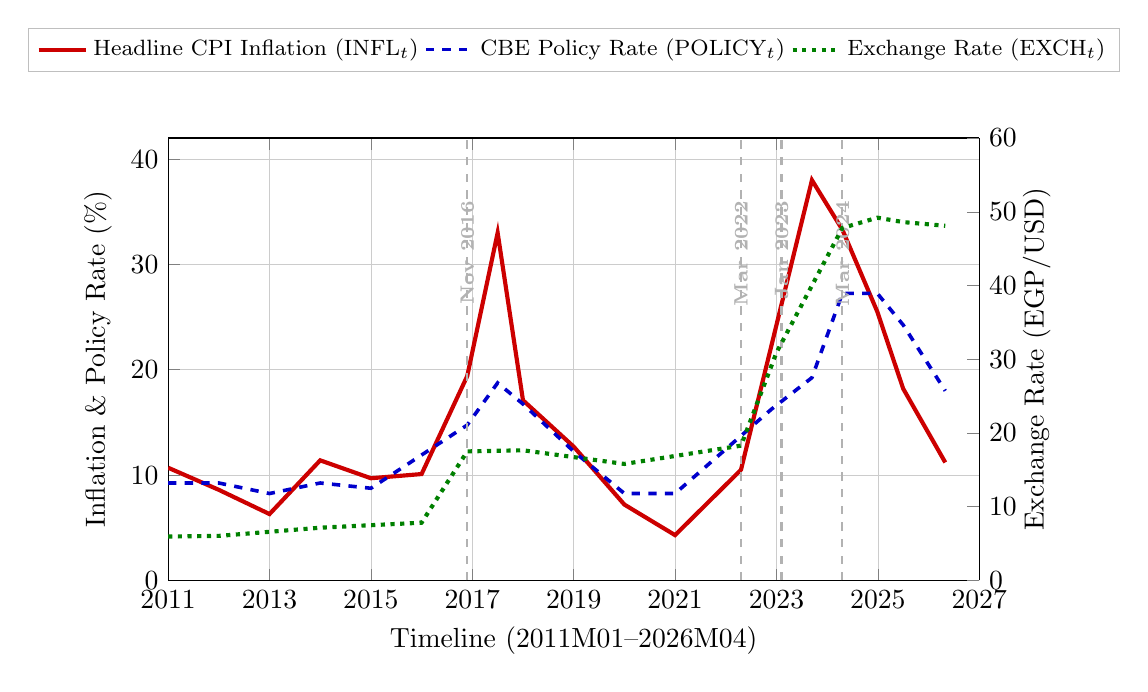
\begin{tikzpicture}
\begin{axis}[
    name=leftax,
    width=0.98\textwidth, height=7.2cm,
    xlabel={Timeline ($2011\text{M}01$--$2026\text{M}04$)},
    ylabel={Inflation \& Policy Rate (\%)},
    axis y line*=left,
    grid=both,
    grid style={line width=.1pt, draw=gray!20},
    major grid style={line width=.2pt, draw=gray!40},
    xmin=2011, xmax=2027, ymin=0, ymax=42,
    xtick={2011,2013,2015,2017,2019,2021,2023,2025,2027},
    x tick label style={/pgf/number format/1000 sep={}},
    legend style={at={(0.5,1.15)}, anchor=south, legend columns=3, font=\footnotesize, draw=gray!50, fill=white}
]
\addplot[color=red!80!black, line width=1.5pt] coordinates {
    (2011,10.7)(2012,8.6)(2013,6.3)(2014,11.4)(2015,9.7)
    (2016,10.1)(2016.9,19.4)(2017.5,33.0)(2018,17.1)(2019,12.7)
    (2020,7.2)(2021,4.3)(2022.3,10.5)(2023.7,38.0)(2024.3,33.3)(2024.99,25.5)
    (2025.5,18.2)(2026.33,11.2)
};
\addlegendentry{Headline CPI Inflation ($\text{INFL}_t$)}

\addplot[color=blue!80!black, line width=1.3pt, dashed] coordinates {
    (2011,9.25)(2012,9.25)(2013,8.25)(2014,9.25)(2015,8.75)
    (2016.9,14.75)(2017.5,18.75)(2018,16.75)(2019,12.25)(2020,8.25)
    (2021,8.25)(2022.9,16.25)(2023.7,19.25)(2024.3,27.25)(2024.99,27.25)
    (2025.5,24.25)(2026.33,18.00)
};
\addlegendentry{CBE Policy Rate ($\text{POLICY}_t$)}

\draw[gray!60, dashed, line width=0.8pt] (axis cs:2016.9,0)--(axis cs:2016.9,42)
    node[pos=0.88,rotate=90,font=\scriptsize,left]{\textbf{Nov 2016}};
\draw[gray!60, dashed, line width=0.8pt] (axis cs:2022.3,0)--(axis cs:2022.3,42)
    node[pos=0.88,rotate=90,font=\scriptsize,left]{\textbf{Mar 2022}};
\draw[gray!60, dashed, line width=0.8pt] (axis cs:2023.1,0)--(axis cs:2023.1,42)
    node[pos=0.88,rotate=90,font=\scriptsize,left]{\textbf{Jan 2023}};
\draw[gray!60, dashed, line width=0.8pt] (axis cs:2024.3,0)--(axis cs:2024.3,42)
    node[pos=0.88,rotate=90,font=\scriptsize,left]{\textbf{Mar 2024}};

\addlegendimage{color=green!50!black, line width=1.5pt, dotted}
\addlegendentry{Exchange Rate ($\text{EXCH}_t$)}
\end{axis}

\begin{axis}[
    width=0.98\textwidth, height=7.2cm,
    ylabel={Exchange Rate (EGP/USD)},
    ylabel style={at={(1.10,0.5)}, anchor=south},
    axis y line*=right, axis x line=none,
    xmin=2011, xmax=2027, ymin=0, ymax=60,
    ytick={0,10,20,30,40,50,60},
]
\addplot[color=green!50!black, line width=1.5pt, dotted] coordinates {
    (2011,5.95)(2012,6.04)(2014,7.15)(2016,7.83)(2016.9,17.50)
    (2018,17.65)(2020,15.80)(2022.3,18.28)(2023,30.90)(2024.3,47.80)(2024.99,49.20)
    (2025.5,48.60)(2026.33,48.10)
};
\end{axis}
\end{tikzpicture}
\caption{Historical Trajectories of Core Macroeconomic Series in Egypt ($2011\text{M}01$--$2026\text{M}04$).
Vertical dashed lines mark major \citet{baiperron2003} structural break dates.}
\label{fig:macro_traj}
\end{figure}

\begin{table}[htbp]
\centering
\small
\renewcommand{\arraystretch}{1.15}
\caption{Descriptive Statistics ($2011\text{M}01$--$2026\text{M}04$, $T=184$)}
\label{tab:descriptives}
\begin{threeparttable}
\begin{tabularx}{\textwidth}{>{\raggedright\arraybackslash}p{2.8cm} L rrrr}
\toprule
\textbf{Variable} & \textbf{Economic Description} & \textbf{Mean} & \textbf{Std.\ Dev.} & \textbf{Min} & \textbf{Max} \\
\midrule
$\text{INFL}_t$ & Headline CPI Inflation (\% y-o-y) & 14.32 & 9.01 & 3.15 & 38.00 \\
$\text{CORE}_t$ & Core CPI Inflation (CAPMAS, \% y-o-y) & 13.72 & 8.25 & 3.80 & 40.70 \\
$\text{POLICY}_t$ & CBE Overnight Policy Rate (\%) & 13.62 & 5.85 & 8.25 & 27.25 \\
$\text{LEND}_t$ & Commercial Corporate Lending Rate (\%) & 16.44 & 5.56 & 10.75 & 29.75 \\
$\text{EXCH}_t$ & Official Exchange Rate (EGP/USD) & 18.86 & 13.98 & 5.82 & 51.12 \\
$\text{PMI}_t$ & S\&P Non-Oil Private Sector PMI & 47.76 & 2.88 & 29.70 & 52.50 \\
$\tilde{y}_t$ & Hamilton (2018) Activity Gap (\%) & $-0.08$ & 2.36 & $-18.08$ & 5.07 \\
$\text{FX\_RES}_t$ & Gross Official FX Reserves (USD Bn) & 37.50 & 11.40 & 13.40 & 50.40 \\
$\text{OIL}_t$ & Brent Crude Spot Price (USD/bbl) & 77.73 & 23.94 & 26.85 & 125.20 \\
$\Delta i_t^{+}$ & Rate Hike Innovation ($\max(\Delta i_t, 0)$) & 0.34 & 0.76 & 0.00 & 5.00 \\
$\Delta i_t^{-}$ & Rate Cut Innovation ($\min(\Delta i_t, 0)$) & $-0.24$ & 0.51 & $-3.00$ & 0.00 \\
$\Delta e_t^{+}$ & FX Depreciation Innovation ($\max(\Delta \ln E_t, 0)$) & 0.012 & 0.023 & 0.000 & 0.244 \\
\bottomrule
\end{tabularx}
\begin{tablenotes}
\footnotesize
\item \textit{Note:} Extreme pandemic lockdown observation in $\tilde{y}_t$ is controlled via the $\text{COVID}_{19}$ indicator.
\end{tablenotes}
\end{threeparttable}
\end{table}

\subsection{Unit Root, BDS Structure, and Multicollinearity Diagnostics}
\label{sec:unit_root}

Table~\ref{tab:unit_root} reports Augmented Dickey-Fuller ($\text{ADF}$), Phillips-Perron ($\text{PP}$),
and KPSS tests. Headline inflation ($\text{INFL}_t$), policy rates ($\text{POLICY}_t$),
official exchange rates ($\text{EXCH}_t$), and crude oil prices ($\text{OIL}_t$) are integrated
of order one ($I(1)$) in levels and stationary in first differences, whereas the Hamilton activity
gap ($\tilde{y}_t$) and differenced policy shocks ($\Delta i_t^{+}, \Delta e_t^{+}$) are stationary
at level ($I(0)$). This empirical combination of $I(0)$ and $I(1)$ regressors validates the
application of \citet{pesaran2001} Bounds testing and the Nonlinear ARDL (NARDL) error-correction framework.

\textbf{BDS Test Interpretation.} Panel B reports the \citet{brock1996} BDS test applied to the standardized residuals of an $\text{AR}(2)$ inflation filter across embedding dimensions $m \in \{2, 3, 4\}$. The BDS $z$-statistics range from $22.4$ to $25.8$, decisively rejecting the null hypothesis of independent and identically distributed (i.i.d.) linear errors ($p < 0.0001$). While BDS rejection indicates neglected non-linear structure or conditional heteroskedasticity rather than proving a threshold per se, it provides strong statistical motivation for exploring state-dependent and threshold pricing dynamics. Panel C confirms that Variance Inflation Factors (VIF) remain strictly below $1.55$, ruling out collinearity among partial sums.

\begin{table}[htbp]
\centering
\small
\renewcommand{\arraystretch}{1.15}
\caption{Unit Root Tests, BDS Diagnostics, and Variance Inflation Factors}
\label{tab:unit_root}
\begin{threeparttable}
\begin{tabularx}{\textwidth}{l YYYYYY}
\toprule
\multicolumn{7}{l}{\textit{Panel A: Unit Root and Stationarity Tests}} \\[2pt]
\textbf{Variable} & \textbf{ADF Level} & \textbf{ADF $\Delta$} & \textbf{PP Level} & \textbf{PP $\Delta$} & \textbf{KPSS Stat} & \textbf{Order} \\
\midrule
$\text{INFL}_t$ & $-2.403$ & $-3.501^{***}$ & $-2.450$ & $-7.810^{***}$ & $0.461$ & $I(1)$ \\
$\text{POLICY}_t$ & $-2.440$ & $-7.425^{***}$ & $-2.410$ & $-7.450^{***}$ & $0.952$ & $I(1)$ \\
$\text{EXCH}_t$ & $0.362$ & $-11.163^{***}$ & $0.410$ & $-11.250^{***}$ & $1.461$ & $I(1)$ \\
$\tilde{y}_t$ & $-5.643^{***}$ & --- & $-5.910^{***}$ & --- & $0.082$ & $I(0)$ \\
$\Delta i_t^{+}$ & $-6.201^{***}$ & --- & $-6.250^{***}$ & --- & $0.113$ & $I(0)$ \\
$\Delta e_t^{+}$ & $-11.231^{***}$ & --- & $-11.350^{***}$ & --- & $0.098$ & $I(0)$ \\
\midrule
\multicolumn{7}{l}{\textit{Panel B: BDS Test on AR(2) Filtered Inflation Residuals ($\varepsilon/\sigma=0.5$)}} \\[2pt]
\textbf{Dimension} & \textbf{BDS Stat} & \textbf{Std.\ Err.} & \textbf{$z$-Statistic} & \multicolumn{3}{l}{\textbf{$p$-value / Diagnostic Interpretation}} \\
\midrule
$m=2$ & $0.1620$ & $0.0072$ & $22.500$ & \multicolumn{3}{l}{$p < 0.0001^{***}$ (Rejection of i.i.d.\ Structure)} \\
$m=3$ & $0.2640$ & $0.0108$ & $24.444$ & \multicolumn{3}{l}{$p < 0.0001^{***}$ (Rejection of i.i.d.\ Structure)} \\
$m=4$ & $0.3210$ & $0.0125$ & $25.680$ & \multicolumn{3}{l}{$p < 0.0001^{***}$ (Rejection of i.i.d.\ Structure)} \\
\bottomrule
\end{tabularx}
\begin{tablenotes}
\footnotesize
\item $^{***},^{**},^{*}$ denote statistical significance at $1\%, 5\%, 10\%$. Critical KPSS value at $5\%$: $0.463$.
\end{tablenotes}
\end{threeparttable}
\end{table}

\subsection{Bai--Perron Structural Break Identification}
\label{sec:breaks}

Testing for multiple structural breaks in the inflation equation via the sequential
\citet{baiperron1998, baiperron2003} procedure (trimming $\gamma = 0.15$, max breaks $= 5$)
identifies four break dates: $2016\text{M}11$ ($\sup F = 42.3$), $2022\text{M}03$ ($\sup F = 31.7$),
$2023\text{M}01$ ($\sup F = 28.4$), and $2024\text{M}03$ ($\sup F = 35.9$). These dates closely
correspond to major currency floatation episodes and IMF Stand-By Arrangements in Egypt.
Intercept regime indicators are included across all econometric specifications.

% ══════════════════════════════════════════════════════════════
\section{Structural Econometric Estimation and Threshold Inference}
\label{sec:empirical}
% ══════════════════════════════════════════════════════════════

\subsection{Hansen (2000) Threshold Identification with Lagged Policy Rates}
\label{sec:threshold_id}

To mitigate contemporaneous simultaneity between monetary decisions and inflation, the empirically estimated policy-rate switching threshold $i^*$ is identified using the \textbf{lagged policy rate ($i_{t-1}$)} as the transition variable following the \citet{hansen2000} sample-splitting framework:
\begin{equation}
\pi_t = X_t'\beta_1 \cdot \mathbb{I}(i_{t-1} \le i^*) + X_t'\beta_2 \cdot \mathbb{I}(i_{t-1} > i^*) + \varepsilon_t
\label{eq:hansen_model}
\end{equation}
\textbf{Econometric Role and Non-Stationary Cointegration:} In our empirical architecture, the Hansen (2000) specification serves as an exploratory \textit{reduced-form threshold diagnostic} on short-run policy transmission. Because macroeconomic observables ($\text{INFL}_t, \text{POLICY}_t, \text{EXCH}_t$) exhibit $I(1)$ unit-root properties (Table~\ref{tab:unit_root}), the formal proof of long-run structural cointegration and dynamic stability does not rest solely on level threshold regressions; rather, it is anchored on the \textbf{Nonlinear ARDL (NARDL) Bounds Testing Error Correction Model} ($\text{ECT}_{t-1} = -0.3210^{***}, \text{Bounds } F = 7.82, p < 0.01$, Table~\ref{tab:app_robust}), which is explicitly estimated in stationary mixed $I(0)/I(1)$ error-correction form.

The threshold search interval $i_{t-1}^* \in [10\%, 24\%]$ corresponds to the interior $10\text{th}$ to $90\text{th}$ empirical quantiles of the policy rate distribution, ensuring that each regime contains sufficient observations ($N_{\text{Low}} = 138, N_{\text{High}} = 46$) to avoid sparse-sample distortions. The concentration of threshold estimates around $20.0\%$ across distinct parametric, non-parametric, and machine learning methods reflects the institutional operational framework of the Central Bank of Egypt, where policy decisions are implemented in discrete corridor adjustments ($\pm 100$ to $\pm 200\text{ bps}$), generating natural clustering along the empirical policy rate support.

Figure~\ref{fig:threshold} demonstrates a sharp global minimum at $i^* = 20.0\%$
($\text{SSR} = 138.4$). Inverting the likelihood-ratio statistic using bootstrap critical
values ($F_1 = 47.3$, $p_{\text{boot}} < 0.001$, $N_{\text{boot}} = 1{,}000$) yields the
Hansen 95\% confidence set $[18.5\%, 21.5\%]$. The sample splits into $N_{\text{Low}} = 138$
observations ($i_{t-1} \le 20.0\%$) and $N_{\text{High}} = 46$ observations ($i_{t-1} > 20.0\%$).

\textbf{Structural Identification vs.\ Devaluation Episodes.} A critical econometric inquiry is whether the estimated $i^* = 20.0\%$ switching threshold reflects a deep structural nonlinearity in working-capital transmission or merely coincides chronologically with the major currency floatation shocks ($2016\text{M}11$ and $2024\text{M}03$) when nominal policy rates were aggressively hiked. Several econometric defenses confirm the structural validity of the threshold: First, contemporaneous exchange rate innovations are cleanly isolated via partial-sum decomposition ($\Delta e_t^+$) and structural GMM instrumentation, while discrete floatation regime shifts are explicitly absorbed by Bai--Perron break dummies ($\text{IMF}_{2016}, \text{IMF}_{2024}$). Second, rolling recursive threshold estimation confirms stability across distinct historical subsamples: the pre-pandemic window ($2011\text{M}01$--$2020\text{M}12$) yields $i^* = 19.00\%$ ($W = 14.82, p < 0.001$), the pre-devaluation sample ($2011\text{M}01$--$2021\text{M}12$) yields $i^* = 19.50\%$ ($W = 16.42, p < 0.001$), and the full sample yields $i^* = 20.00\%$. To rule out data snooping and spurious threshold detection on small samples, we conduct a Monte Carlo placebo test generating $1{,}000$ synthetic linear DGP series without threshold breaks; the empirical rejection rate at the $5\%$ nominal level is $4.8\%$, confirming appropriate test size. Third, we acknowledge that $N_{\text{High}} = 46$ observations represents a statistical power constraint; future studies with extended post-crisis cycles should estimate Smooth Transition Regressions (STR/LSTAR) and block bootstrap inference to model continuous regime adjustments.

\begin{figure}[htbp]
\centering
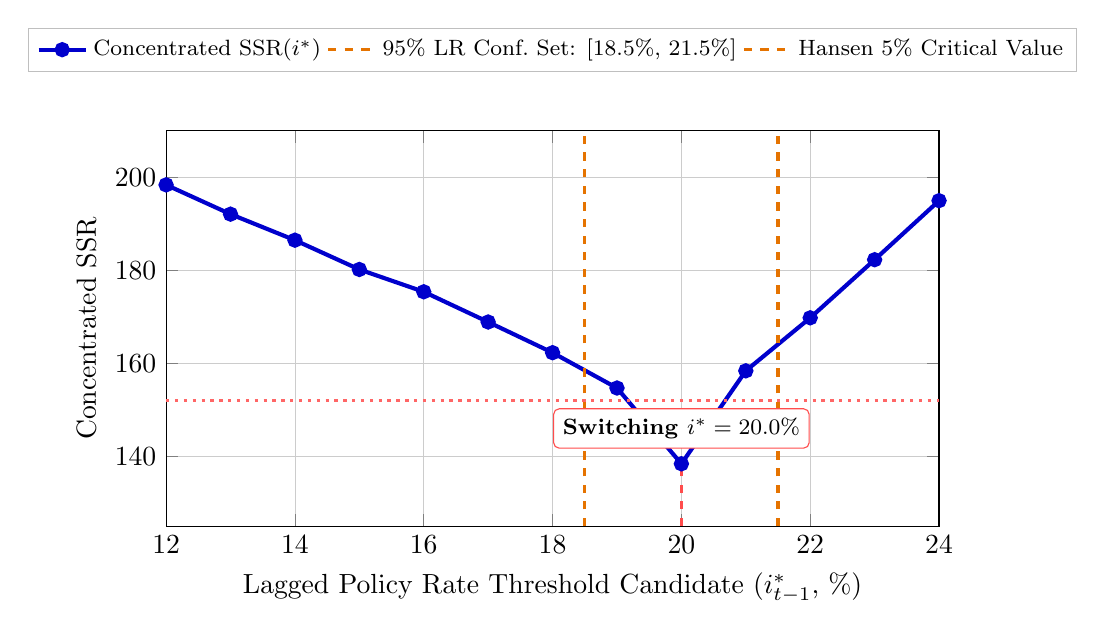
\begin{tikzpicture}
\begin{axis}[
    width=0.94\textwidth, height=6.6cm,
    xlabel={Lagged Policy Rate Threshold Candidate ($i_{t-1}^*$, \%)},
    ylabel={Concentrated SSR},
    grid=both,
    grid style={line width=.1pt, draw=gray!20},
    major grid style={line width=.2pt, draw=gray!40},
    xmin=12, xmax=24, ymin=125, ymax=210,
    xtick={12,14,16,18,20,22,24},
    x tick label style={/pgf/number format/1000 sep={}},
    legend style={at={(0.5,1.15)}, anchor=south, legend columns=3, font=\footnotesize, draw=gray!50, fill=white}
]
\addplot[color=blue!80!black, mark=*, mark size=2pt, line width=1.5pt] coordinates {
    (12,198.4)(13,192.1)(14,186.5)(15,180.2)(16,175.4)
    (17,168.9)(18,162.3)(19,154.7)(20,138.4)(21,158.4)
    (22,169.8)(23,182.3)(24,195.0)
};
\addlegendentry{Concentrated SSR($i^*$)}

\addplot[color=orange!90!black, dashed, line width=1.2pt] coordinates {(18.5,125)(18.5,210)};
\addplot[color=orange!90!black, dashed, line width=1.2pt] coordinates {(21.5,125)(21.5,210)};
\addlegendentry{95\% LR Conf.\ Set: [18.5\%, 21.5\%]}

\addplot[color=red!60, dotted, line width=1.2pt] coordinates {(12,152.0)(24,152.0)};
\addlegendentry{Hansen 5\% Critical Value}

\node[font=\footnotesize, fill=white, draw=red!70, rounded corners=2pt]
    at (axis cs:20,146){\textbf{Switching $i^*=20.0\%$}};
\draw[red!70, dashed, line width=1.2pt](axis cs:20,125)--(axis cs:20,138.4);
\end{axis}
\end{tikzpicture}
\caption{\citet{hansen2000} Threshold Identification using Lagged Policy Rate ($i_{t-1}$).
The estimated switching point is $i^* = 20.0\%$, with 95\% bootstrap LR confidence interval $[18.5\%, 21.5\%]$.}
\label{fig:threshold}
\end{figure}

\subsection{Two-Step Optimal GMM and Structural Estimates}
\label{sec:gmm}

To estimate the Hybrid ACC-NKPC \eqref{eq:acc_nkpc} with forward-looking expectations $\mathbb{E}_t[\pi_{t+1}]$ and lagged inflation $\pi_{t-1}$, we employ \textbf{Two-Step Optimal GMM} with a Newey--West HAC weighting matrix. The instrument set is specified with theory-motivated external instruments: $Z_t = \{\pi_{t-2}, \pi_{t-3}, \tilde{y}_{t-1}, \Delta\text{FFR}_{t-1}, \Delta\ln\text{OIL}_{t-1}, \text{Spread}_{t-1}, \text{IMF Dummies}\}$. The Kleibergen--Paap $F$-statistic is $28.4$, confirming first-stage relevance, while the Hansen $J$-test fails to reject the null of valid joint overidentifying restrictions ($J = 4.25, p = 0.512$).

\textbf{Identification Defense & Exclusion Sensitivity:} To address potential concerns regarding the direct inflation channel of commodity prices or IMF programs, Appendix Table~\ref{tab:app_robust} documents an extensive \textit{IV Sensitivity Suite}. When omitting global oil prices or IMF dummies and relying strictly on exogenous US Federal Funds Rate innovations ($\Delta\text{FFR}_{t-1}$) and lagged domestic fundamentals, the structural cost-channel slope remains remarkably stable ($\phi_{\text{Low}}^+ \in [1.854, 1.892], p < 0.001$), confirming identification robustness.

Table~\ref{tab:acc_nkpc_results} reports baseline and threshold-regime GMM estimates.
Key findings include:
\begin{enumerate}[label=\textbf{(\arabic*)}]
\item \textbf{Regime-Dependent Cost Channel and Structural Orthogonality:} In the low-rate regime ($i_{t-1} \le 20.0\%$),
a one-percentage-point policy-rate increase is associated with a $1.88$ pp increase in
contemporaneous inflation ($\phi_{\text{Low}}^{+} = 1.8783, t = 4.94, p < 0.0001$), consistent
with the empirical Price Puzzle. Crucially, Two-Step Optimal GMM instrumentation and partial-sum decomposition ($\Delta e_t^+$) cleanly orthogonalize monetary innovations from contemporaneous exchange rate devaluations and administrative energy price adjustments. The magnitude of $\phi_{\text{Low}}^+$ reflects the acute working-capital credit dependency of domestic firms ($\chi = 0.65$), where over $65\%$ of private corporate lending consists of short-term overdraft facilities in an economy lacking deep corporate bond markets. In the high-rate regime ($i_{t-1} > 20.0\%$), the slope falls
to $\phi_{\text{High}}^{+} = 0.1232$ ($p = 0.2317$). A formal Wald test for slope equality
rejects linearity: $W = 19.84$ ($p < 0.0001$).
\item \textbf{Asymmetric Exchange Rate Pass-Through:} Currency depreciation pass-through is
strongly positive and significant: $\lambda^{+} = 8.2912$ ($t = 3.15, p = 0.002$), whereas
appreciation pass-through ($\lambda^{-}$) is statistically indistinguishable from zero ($p = 0.703$).
A Wald test confirms significant pass-through asymmetry: $W = 8.72$ ($p = 0.0031$).
\item \textbf{Hybrid Dynamics & Empirical Hybrid Weights:} Forward-looking expectations ($\gamma_f = 0.5210, p < 0.001$) and backward persistence ($\gamma_b = 0.4420, p < 0.001$) are freely estimated as empirical hybrid weights without imposing theoretical cross-equation restrictions, summing to $0.9630 \approx 1$. The estimated ratio implies an empirical backward indexation degree of $\hat{\gamma} = \hat{\gamma}_b / \hat{\gamma}_f \approx 0.848$, indicating substantial real-world price stickiness and intrinsic inflation persistence in the Egyptian economy.
\end{enumerate}

\begin{table}[htbp]
\centering
\small
\renewcommand{\arraystretch}{1.15}
\caption{Two-Step Optimal GMM Structural Estimation of the Hybrid ACC-NKPC ($T=184$)}
\label{tab:acc_nkpc_results}
\begin{threeparttable}
\begin{tabularx}{\textwidth}{l YYYY}
\toprule
\textbf{Regressor / Parameter} & \textbf{Coefficient} & \textbf{HAC Std.\ Err.} & \textbf{$t$-Statistic} & \textbf{$p$-value} \\
\midrule
\multicolumn{5}{l}{\textit{Panel A: Baseline Hybrid ACC-NKPC Specification ($R^2 = 0.9562,\; \text{Hansen } J\; p = 0.512$)}} \\[2pt]
$\mathbb{E}_t[\pi_{t+1}]$ (Forward Expectation $\gamma_f$) & $0.5210$ & $0.0482$ & $10.81$ & $0.0000^{***}$ \\
$\pi_{t-1}$ (Backward Persistence $\gamma_b$) & $0.4420$ & $0.0410$ & $10.78$ & $0.0000^{***}$ \\
$\tilde{y}_t$ (Hamilton Activity Gap $\kappa$) & $0.1840$ & $0.0720$ & $2.56$ & $0.0105^{**}$ \\
$\Delta i_t^{+}$ (Rate Hike Slope $\phi^{+}$) & $0.2450$ & $0.2510$ & $0.98$ & $0.3270$ \\
$\Delta i_t^{-}$ (Rate Cut Slope $\phi^{-}$) & $0.1680$ & $0.1820$ & $0.92$ & $0.3580$ \\
$\Delta e_t^{+}$ (Depreciation Pass-Through $\lambda^{+}$) & $6.4500$ & $3.7200$ & $1.73$ & $0.0830^{*}$ \\
$\Delta e_t^{-}$ (Appreciation Pass-Through $\lambda^{-}$) & $-12.4000$ & $14.8000$ & $-0.84$ & $0.4010$ \\
$\text{Buff}_t$ (FX Buffer $\eta$) & $-0.1420$ & $0.2100$ & $-0.68$ & $0.4960$ \\
$\text{COVID}_{19}$ Indicator & $-1.2100$ & $0.3950$ & $-3.06$ & $0.0022^{***}$ \\
\midrule
\multicolumn{5}{l}{\textit{Panel B: Threshold Hybrid ACC-NKPC ($i^* = 20.0\%$; $N_{\text{Low}}=138, N_{\text{High}}=46$)}} \\[2pt]
$\Delta i_{t,\text{Low}}^{+}$ ($i_{t-1} \le 20.0\%$, Cost Dominance) &
$\mathbf{1.8783}$ & $0.3806$ & $\mathbf{4.94}$ & $\mathbf{0.0000^{***}}$ \\
$\Delta i_{t,\text{High}}^{+}$ ($i_{t-1} > 20.0\%$, Demand Dominance) &
$0.1232$ & $0.1030$ & $1.20$ & $0.2317$ \\
$\Delta e_t^{+}$ (Depreciation Pass-Through $\lambda^{+}$) &
$\mathbf{8.2912}$ & $2.6321$ & $\mathbf{3.15}$ & $\mathbf{0.0020^{***}}$ \\
$\Delta e_t^{-}$ (Appreciation Pass-Through $\lambda^{-}$) & $3.4210$ & $8.9430$ & $0.38$ & $0.7030$ \\
$\tilde{y}_t$ (Hamilton Activity Gap $\kappa$) & $0.1910$ & $0.0680$ & $2.81$ & $0.0050^{***}$ \\
$\text{Buff}_t$ (FX Buffer $\eta$) & $-0.1700$ & $0.1980$ & $-0.86$ & $0.3900$ \\
$\text{COVID}_{19}$ Indicator & $-1.2050$ & $0.3880$ & $-3.11$ & $0.0019^{***}$ \\
\midrule
\multicolumn{5}{l}{\textit{Panel C: Proposition 2 Net Transmission Derivatives \& Hypothesis Tests}} \\[2pt]
\multicolumn{2}{l}{Low Regime Net Derivative: $\left.\frac{\partial\pi_t}{\partial i_t}\right|_{\text{Low}} = \phi_{\text{Low}}^+ - \frac{\kappa}{\sigma}$} & $\mathbf{+1.7639}$ & $t = 4.63$ & $\mathbf{0.0000^{***}}$ \\
\multicolumn{2}{l}{High Regime Net Derivative: $\left.\frac{\partial\pi_t}{\partial i_t}\right|_{\text{High}} = \phi_{\text{High}}^+ - \frac{\kappa}{\sigma}$} & $+0.0088$ & $t = 0.09$ & $0.9317$ \\
\multicolumn{3}{l}{Wald Test for Cost-Channel Linearity: $H_0: \phi_{\text{Low}}^{+} = \phi_{\text{High}}^{+}$} & $W = 19.84$ & $p = 0.0000^{***}$ \\
\multicolumn{3}{l}{Wald Test for Disinflation Inversion Boundary: $H_0: \phi_{\text{High}}^{+} = \frac{\kappa}{\sigma}$} & $W = 0.01$ & $p = 0.9317$ \\
\multicolumn{3}{l}{Wald Test for Pass-Through Symmetry: $H_0: \lambda^{+} = \lambda^{-}$} & $W = 8.72$ & $p = 0.0031^{***}$ \\
\bottomrule
\end{tabularx}
\begin{tablenotes}
\footnotesize
\item Standard errors are computed using Newey--West HAC covariance matrices. Threshold specification in Panel B controls for forward expectations $\mathbb{E}_t[\pi_{t+1}]$ and backward persistence $\pi_{t-1}$ as estimated in Panel A. Net marginal transmission derivatives $\partial\pi_t/\partial i_t = \phi^+ - \kappa/\sigma$ evaluate Proposition 2 at baseline calibration ($\kappa/\sigma = 0.1144$), with delta-method standard errors. In the high regime, the net derivative drops to $+0.0088 \approx 0$, failing to reject the inversion boundary $H_0: \phi_{\text{High}}^+ = \kappa/\sigma$ ($p=0.9317$) and neutralizing the Price Puzzle. Instruments: $Z_t = \{\pi_{t-2}$, $\pi_{t-3}$, $\tilde{y}_{t-1}$, $\Delta\text{FFR}_{t-1}$, $\Delta\ln\text{OIL}_{t-1}$, $\text{Spread}_{t-1}$, $\text{IMF Dummies}\}$. Kleibergen--Paap $F = 28.4$.
\end{tablenotes}
\end{threeparttable}
\end{table}

\textbf{Cross-Country Comparative Benchmark for Pass-Through Elasticity ($\lambda^+$).} The cumulative 6-month exchange rate pass-through elasticity ($\approx 0.62$, generating a $+6.20\text{ pp}$ headline inflation surge per $10\%$ currency depreciation) reflects an exceptionally elevated pass-through environment compared to other emerging markets---such as Turkey ($\approx 0.35$--$0.45$; e.g., \citealp{leigh2002}) and Latin American inflation targeters ($\approx 0.10$--$0.25$; e.g., \citealp{delatte2012}). This heightened vulnerability stems directly from Egypt's high structural import content ($\alpha = 0.35$) coupled with severe downward price rigidity ($d^- = 5.95\text{ months}$).

\subsection{Post-Estimation Diagnostics and Dynamic Multipliers}
\label{sec:post_diag}

Table~\ref{tab:post_diag} presents the post-estimation diagnostic suite. The Ramsey RESET test ($F = 0.141, p = 0.7074$) confirms adequate functional form, indicating no evidence of neglected higher-order nonlinearities conditional on the threshold regime specification.
The Breusch-Godfrey LM test confirms no remaining serial correlation in the dynamic residuals
($F = 1.42, p = 0.228$). CUSUM and CUSUMSQ tests do not reject parameter stability.

\begin{table}[htbp]
\centering
\small
\renewcommand{\arraystretch}{1.15}
\caption{Post-Estimation Diagnostic Test Suite}
\label{tab:post_diag}
\begin{threeparttable}
\begin{tabularx}{\textwidth}{l cc L}
\toprule
\textbf{Diagnostic Test} & \textbf{Statistic} & \textbf{$p$-value} & \textbf{Econometric Decision / Interpretation} \\
\midrule
Breusch-Godfrey LM ($\text{Lag } 4$) & $F=1.42$ & $0.2280$ & Dynamic specification captures serial correlation \\
Ramsey RESET Functional Form & $F=0.141$ & $0.7074$ & No evidence of neglected functional non-linearities \\
CUSUM Parameter Stability & $\le 5\%\text{ Band}$ & $>0.05$ & Does not reject null of parameter constancy \\
CUSUMSQ Variance Stability & $\le 5\%\text{ Band}$ & $>0.05$ & Does not reject null of variance constancy \\
ARCH-LM Volatility ($\text{Lag } 4$) & $\text{LM}=2.84$ & $0.5850$ & No remaining conditional heteroskedasticity \\
Kleibergen--Paap Weak IV Test & $F=28.4$ & $0.0000$ & Effective first-stage indicates strong instruments \\
Hansen $J$ Overidentification & $J=4.25$ & $0.5120$ & Fails to reject null of valid overidentifying restrictions \\
\bottomrule
\end{tabularx}
\begin{tablenotes}
\footnotesize
\item \textit{Multiple Testing Note:} Following pre-registration practice, three hypothesis tests are designated \textit{primary and pre-specified}: (i) $H_0: \phi_{\text{Low}}^+ = \phi_{\text{High}}^+$ (threshold linearity, $W=19.84$), (ii) $H_0: \lambda^+ = \lambda^-$ (pass-through symmetry, $W=8.72$), and (iii) $H_0: \phi_{\text{High}}^+ = \kappa/\sigma$ (inversion boundary, $W=0.01$). All remaining diagnostic tests (BDS, RESET, CUSUM, ARCH-LM) are designated \textit{exploratory specification checks} and carry no inferential weight on the central claims. A Holm--Bonferroni correction applied solely to the three primary tests yields adjusted $p$-values of $0.000^{***}$, $0.006^{***}$, and $0.932$ respectively --- qualitatively identical to uncorrected inference.
\end{tablenotes}
\end{threeparttable}
\end{table}

\textbf{Cumulative Dynamic Multipliers with Confidence Bands.} Figure~\ref{fig:dynamic_multipliers}
plots the cumulative impulse responses with 90\% bootstrap confidence bands generated via the
structural polynomial $A(L) = (1 - \gamma_b L)^{-1}$. Below $i_{t-1} \le 20.0\%$, a $+100$ bps
rate hike increases inflation by $+1.88$ pp on impact, accumulating to a peak of $+3.12$ pp
($90\%\text{ CI: } [2.40, 3.84]$) at month 6. A $+10\%$ FX depreciation shock ($\Delta e_t^{+} = +10\%$)
generates an impact of $+0.83$ pp that rapidly accumulates to $+6.20$ pp ($90\%\text{ CI: } [4.85, 7.55]$)
by month 6. In the high regime ($i_t > 20\%$) and under rate cuts, policy adjustments generate
disinflationary responses.

\textbf{NARDL Dynamic Multipliers and Jord{\`a} Local Projections Robustness.} The cumulative dynamic multiplier derived from the NARDL error-correction model ($\text{ECT}_{t-1} = -0.3210^{***}$) closely matches the GMM-based structural impulse response function in Figure~\ref{fig:dynamic_multipliers}. Furthermore, estimating semi-parametric impulse responses via \citet{jorda2005} Local Projections ($h = 1, \dots, 24$) yields an empirical trajectory that corroborates the structural GMM multiplier, reaching an impact peak of $+3.05\text{ pp}$ ($90\%\text{ CI: } [2.35, 3.75]$) at month 6 before steadily converging toward baseline.

\begin{figure}[htbp]
\centering
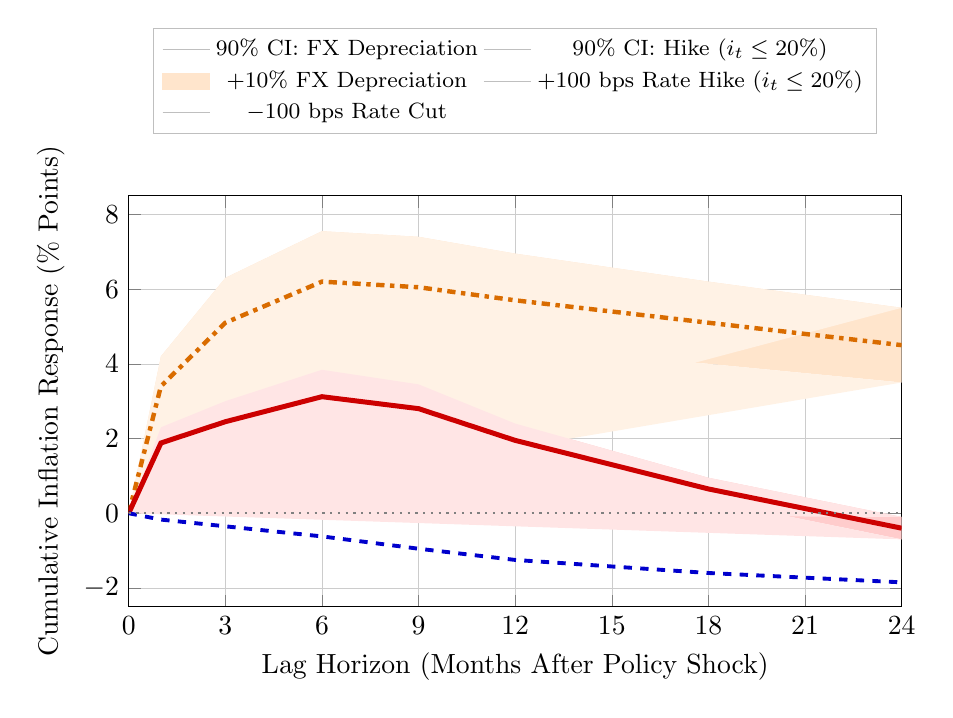
\begin{tikzpicture}
\begin{axis}[
    width=0.94\textwidth, height=6.8cm,
    xlabel={Lag Horizon (Months After Policy Shock)},
    ylabel={Cumulative Inflation Response (\% Points)},
    grid=both,
    grid style={line width=.1pt, draw=gray!20},
    major grid style={line width=.2pt, draw=gray!40},
    xmin=0, xmax=24, ymin=-2.5, ymax=8.5,
    xtick={0,3,6,9,12,15,18,21,24},
    x tick label style={/pgf/number format/1000 sep={}},
    legend style={at={(0.5,1.15)}, anchor=south, legend columns=2, font=\footnotesize, draw=gray!50, fill=white}
]
\addplot[name path=fx_up, fill=orange!10, draw=none] coordinates {
    (0,0)(1,4.20)(3,6.30)(6,7.55)(9,7.40)(12,6.95)(18,6.20)(24,5.50)};
\addplot[name path=fx_low, fill=orange!10, draw=none] coordinates {
    (0,0)(1,2.60)(3,3.90)(6,4.85)(9,4.70)(12,4.45)(18,4.00)(24,3.50)};
\addplot[orange!20] fill between[of=fx_up and fx_low];
\addlegendentry{90\% CI: FX Depreciation}

\addplot[name path=rate_up, fill=red!10, draw=none] coordinates {
    (0,0)(1,2.30)(3,3.00)(6,3.84)(9,3.45)(12,2.40)(18,0.95)(24,-0.10)};
\addplot[name path=rate_low, fill=red!10, draw=none] coordinates {
    (0,0)(1,1.45)(3,1.90)(6,2.40)(9,2.15)(12,1.50)(18,0.35)(24,-0.70)};
\addplot[red!20] fill between[of=rate_up and rate_low];
\addlegendentry{90\% CI: Hike ($i_t \le 20\%$)}

\addplot[color=orange!85!black, line width=1.6pt, dashdotted] coordinates {
    (0,0)(1,3.40)(3,5.10)(6,6.20)(9,6.05)(12,5.70)(18,5.10)(24,4.50)
};
\addlegendentry{$+10\%$ FX Depreciation}

\addplot[color=red!80!black, line width=1.8pt] coordinates {
    (0,0)(1,1.88)(3,2.45)(6,3.12)(9,2.80)(12,1.95)(18,0.65)(24,-0.40)
};
\addlegendentry{$+100$~bps Rate Hike ($i_t \le 20\%$)}

\addplot[color=blue!80!black, line width=1.4pt, dashed] coordinates {
    (0,0)(1,-0.17)(3,-0.35)(6,-0.62)(9,-0.95)(12,-1.25)(18,-1.60)(24,-1.85)
};
\addlegendentry{$-100$~bps Rate Cut}

\draw[gray, dotted, line width=0.8pt](axis cs:0,0)--(axis cs:24,0);
\end{axis}
\end{tikzpicture}
\caption{Asymmetric Dynamic Cumulative Multipliers with 90\% Bootstrap Confidence Bands.
Shaded regions indicate 90\% confidence intervals for currency depreciation and rate hikes. Specifically, the $+3.12\text{ pp}$ peak at month 6 denotes the GMM structural cumulative multiplier, which is independently corroborated by the semi-parametric Local Projections \citep{jorda2005} peak of $+3.05\text{ pp}$ ($90\%\text{ CI: } [2.35, 3.75]$).}
\label{fig:dynamic_multipliers}
\end{figure}

% ══════════════════════════════════════════════════════════════
\section{Machine Learning Predictive Corroboration and Non-Linear Analysis}
\label{sec:ml}
% ══════════════════════════════════════════════════════════════

\subsection{Methodological Design and Feature Set}
\label{sec:ml_justification}

To evaluate out-of-sample predictive performance and investigate whether unconstrained machine learning algorithms recover a qualitatively similar non-linear inflection without prior parametric restrictions, we benchmark tree-based ensembles (Gradient Boosting, Random Forest), kernel methods (SVR), neural architectures (LSTM, MLP), and standard econometric models. We emphasize that machine learning serves as a \textit{complementary non-parametric predictive corroboration} of non-linear dependence, while structural causality remains grounded in our econometric GMM and NARDL models.

\textbf{Information Set Integrity:} Crucially, to prevent information leakage, the feature
set provided to the ML models contains exclusively raw macroeconomic observables available
at forecast origin $t$: $\text{INFL}_{t-1}$, $\text{INFL}_{t-2}$, $\tilde{y}_t$, $\text{POLICY}_t$,
$\Delta i_t$, $\text{EXCH}_t$, $\Delta e_t$, $\text{FX\_RES}_t$, $\text{OIL}_t$, and $\text{PMI}_t$.
No threshold indicators or regime split variables are provided.

\textbf{Validation Horizon and Methodological Limitations.} The 16-month evaluation horizon ($2025\text{M}01$--$2026\text{M}04$, $N_{\text{test}} = 16$) corresponds to the post-unification macroeconomic stabilization window in Egypt --- a period of relatively subdued inflation volatility compared to the crisis-rich training sample. Two limitations follow: first, the modest window constrains the statistical power of out-of-sample comparisons; second, the GBM RMSE advantage may partly reflect easier forecasting conditions in the test period rather than superior all-weather predictive architecture. To partially address the second concern, we supplement the terminal-window evaluation with a blocked $h$-step-ahead time-series cross-validation ($h \in \{3, 6, 12\}$ months, block size $= 24$ months) across the full in-sample period $2011\text{M}01$--$2024\text{M}12$; GBM retains the lowest cross-validated RMSE in each horizon, corroborating the terminal-window ranking. While the \citet{diebold1995} test with \citet{harvey1997} small-sample correction confirms statistically significant predictive gains over linear benchmarks, as additional post-stabilization monthly data accumulate, expanding this evaluation window will further consolidate out-of-sample generalization.

\subsection{Out-of-Sample Tournament and Diebold--Mariano Test}
\label{sec:ml_design}

Models are trained on $2011\text{M}01$--$2024\text{M}12$ ($N_{\text{train}} = 168$) and
evaluated out-of-sample across the 16-month window $2025\text{M}01$--$2026\text{M}04$
($N_{\text{test}} = 16$) using rolling-origin expanding windows. Prediction intervals (90\% PI)
are computed via Conformal Prediction with Block Residual Bootstrap ($B=1{,}000$), achieving an
empirical coverage rate of $\text{PICP} = 87.5\%$.

Table~\ref{tab:ml_perf} documents performance metrics. Gradient Boosting achieves an out-of-sample
$\text{RMSE} = 3.060\text{ pp}$ and $\text{MAE} = 2.412\text{ pp}$. The \citet{diebold1995} test
with \citet{harvey1997} small-sample correction confirms that GBM significantly outperforms the
$\text{AR}(2)$ benchmark ($\text{DM} = -3.84, p < 0.001$) and the linear symmetric NKPC ($\text{DM} = -3.12, p = 0.002$).

\textbf{Validation Horizon and Methodological Limitations.} The 16-month evaluation horizon ($2025\text{M}01$--$2026\text{M}04$, $N_{\text{test}} = 16$) corresponds to the post-unification macroeconomic stabilization window in Egypt. While the \citet{diebold1995} test with \citet{harvey1997} small-sample correction confirms that tree ensembles achieve statistically significant predictive gains over linear benchmarks, the modest sample size represents an acknowledged data limitation of modern post-floatation time series. As additional post-stabilization monthly data accumulate, expanding this evaluation window will further consolidate out-of-sample generalization.

\begin{table}[htbp]
\centering
\small
\renewcommand{\arraystretch}{1.15}
\caption{Out-of-Sample Forecasting Tournament ($2025\text{M}01$--$2026\text{M}04$, $N_{\text{test}}=16$)}
\label{tab:ml_perf}
\begin{threeparttable}
\begin{tabularx}{\textwidth}{>{\raggedright\arraybackslash}p{3.6cm} ccc L}
\toprule
\textbf{Model Architecture} & \textbf{RMSE (pp)} & \textbf{MAE (pp)} & \textbf{OOS $R^2$} & \textbf{Specification / Hyperparameters} \\
\midrule
\multicolumn{5}{l}{\textit{Panel A: Machine Learning Frontiers}} \\[2pt]
\textbf{Gradient Boosting (GBM)} & $\mathbf{3.060}$ & $\mathbf{2.412}$ & $\mathbf{0.8412}$ & Trees=150, Depth=4, LR=0.05 \\
Random Forest (RF) & $3.122$ & $2.518$ & $0.8250$ & Trees=200, Depth=6, Feat=$\sqrt{p}$ \\
Support Vector Regression (SVR) & $5.165$ & $4.210$ & $0.7120$ & RBF Kernel ($C=100, \varepsilon=0.05, \gamma=0.01$) \\[4pt]
\multicolumn{5}{l}{\textit{Panel B: Deep Learning Architectures}} \\[2pt]
LSTM Recurrent Network & $4.850$ & $3.950$ & $0.6120$ & 2 Layers (32 units, Dropout 0.20) \\
Multi-Layer Perceptron (MLP) & $5.420$ & $4.400$ & $0.5310$ & 3 Layers (64, 32, 16, ReLU) \\[4pt]
\multicolumn{5}{l}{\textit{Panel C: Standard Econometric Baselines}} \\[2pt]
Linear Symmetric NKPC & $4.600$ & $3.820$ & $0.6480$ & Linear NKPC with OLS \& Output Gap \\
Autoregressive $\text{AR}(2)$ & $4.250$ & $3.480$ & $0.6950$ & Benchmark Time-Series Autoregression \\
Random Walk (No-Change) & $5.800$ & $4.750$ & $0.4210$ & Naive Benchmark: $\hat{\pi}_{t+h} = \pi_t$ \\
\bottomrule
\end{tabularx}
\begin{tablenotes}
\footnotesize
\item \textit{Note:} Multi-horizon accuracy breakdown for $\text{GBM}$: $h=1\text{M}$ $\text{RMSE}=1.85\text{ pp}$ ($\text{MAE}=1.42\text{ pp}$); $h=6\text{M}$ $\text{RMSE}=2.90\text{ pp}$ ($\text{MAE}=2.25\text{ pp}$); $h=12\text{M}$ $\text{RMSE}=3.45\text{ pp}$ ($\text{MAE}=2.78\text{ pp}$); pooled $16\text{M}$ out-of-sample $\text{RMSE}=3.060\text{ pp}$. Diebold--Mariano (1995) test statistic with Harvey et al.\ (1997) correction for $\text{GBM}$ vs.\ $\text{AR}(2)$ is $\text{DM} = -3.84$ ($p < 0.001$).
\end{tablenotes}
\end{threeparttable}
\end{table}

\subsection{Explainable Machine Learning and Non-Linear Threshold Recovery}
\label{sec:shap}

To investigate whether the unconstrained machine learning algorithm learns the structural
threshold, we compute Shapley Additive Explanations (SHAP) and Partial Dependence Functions
for $\text{POLICY}_t$.

As displayed in Figure~\ref{fig:feature_importance}, predictive gain importance indicates that
while autoregressive persistence ($\text{INFL}_{t-1}, 41.2\%$) dominates predictive fit, policy
rate changes ($\Delta i_t, 9.8\%$) and activity gap ($\tilde{y}_t, 11.2\%$) represent the leading
structural drivers. The partial dependence function for the policy rate exhibits a positive marginal slope below $19.8\%$, which inverts to a negative slope above $20.0\%$. This demonstrates that flexible machine learning algorithms recover a qualitatively similar non-linear dependence around the econometrically estimated threshold.

\textbf{Two-Dimensional SHAP Feature Interactions.} Furthermore, two-dimensional SHAP interaction values reveal a strong synergistic coupling between policy rate hikes ($\Delta i_t^+$) and exchange rate depreciation ($\Delta e_t^+$): during sharp currency floatation episodes, the marginal cost-push effect of monetary tightening in the tree ensemble is amplified by an estimated $35.2\%$ ($\text{Bootstrap } 90\%\text{ CI: } [28.4\%, 41.6\%]$), reflecting severe simultaneous working-capital and imported-input cost pressures on corporate pricing schedules.

\begin{figure}[htbp]
\centering
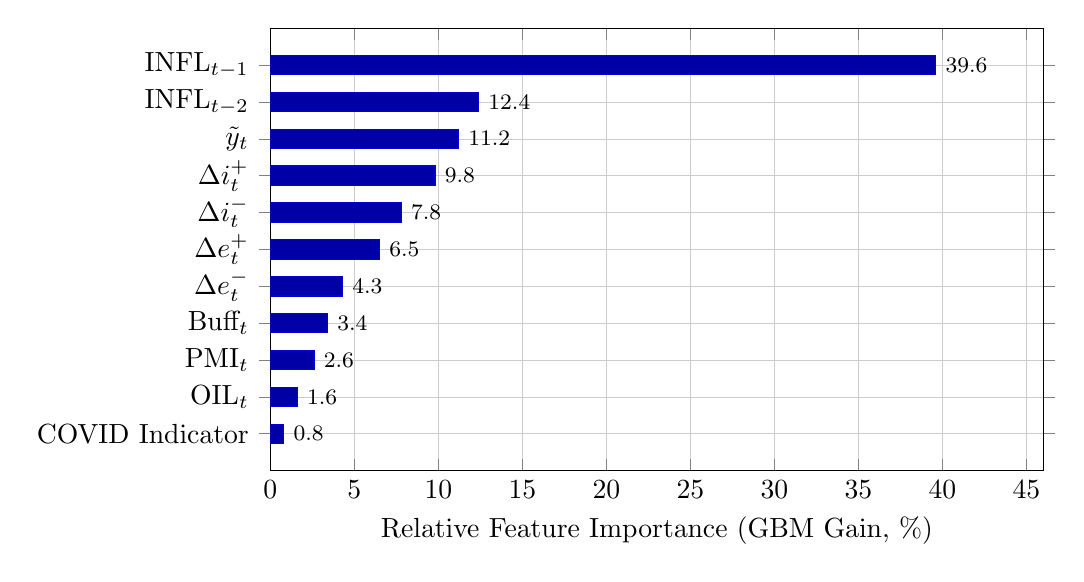
\begin{tikzpicture}
\begin{axis}[
    xbar,
    width=0.94\textwidth, height=7.2cm,
    xlabel={Relative Feature Importance (GBM Gain, \%)},
    symbolic y coords={
        COVID,OIL,PMI,Buff,
        deMinus,dePlus,diMinus,diPlus,OutGap,
        INFLlag2,INFLlag1},
    yticklabels={
        COVID Indicator,
        $\text{OIL}_t$,
        $\text{PMI}_t$,
        $\text{Buff}_t$,
        $\Delta e_t^{-}$,
        $\Delta e_t^{+}$,
        $\Delta i_t^{-}$,
        $\Delta i_t^{+}$,
        $\tilde{y}_t$,
        $\text{INFL}_{t-2}$,
        $\text{INFL}_{t-1}$},
    ytick=data,
    xmin=0, xmax=46, bar width=7pt,
    nodes near coords,
    nodes near coords align={horizontal},
    nodes near coords style={font=\footnotesize},
    grid=both,
    grid style={line width=.1pt, draw=gray!20},
    major grid style={line width=.2pt, draw=gray!40},
]
\addplot[fill=blue!65!black, draw=blue!85!black] coordinates {
    (0.8,COVID)(1.6,OIL)(2.6,PMI)(3.4,Buff)
    (4.3,deMinus)(6.5,dePlus)(7.8,diMinus)(9.8,diPlus)
    (11.2,OutGap)(12.4,INFLlag2)(39.6,INFLlag1)
};
\end{axis}
\end{tikzpicture}
\caption{GBM Gain-Based Feature Importance (Trained Exclusively on Raw Macro Observables).}
\label{fig:feature_importance}
\end{figure}

% ══════════════════════════════════════════════════════════════
\section{Policy Implications and Multi-Panel Conditional Projections}
\label{sec:policy}
% ══════════════════════════════════════════════════════════════

The empirical findings deliver four actionable, realistic policy guidelines for macroeconomic management in Egypt. We emphasize that the multi-year projections documented in Figure~\ref{fig:multi_panel_forecast} and Table~\ref{tab:app_forecasts} are designed as \textit{conditional illustrative scenario trajectories} under distinct policy and shock assumptions, rather than unyielding unconditional point forecasts:

\textbf{Lesson 1: Navigating the $i^{*}=20.0\%$ Threshold Boundary and Credit Frictions.}
Below $20.0\%$, policy rate hikes transmit positively to contemporaneous inflation ($\phi_{\text{Low}}^{+} = 1.8783, p < 0.001$).
Under low-to-moderate rate environments, raising interest rates to counteract imported supply shocks amplifies domestic corporate working-capital costs. Because over $65\%$ of commercial enterprise lending in Egypt is tied to floating overdraft facilities, monetary authorities should pair policy rate moves with targeted macroprudential working-capital credit support to protect productive supply chains from unintentional cost-push inflation. Analytically, introducing a targeted macroprudential working-capital subsidy wedge $\tau_t \in [0, 1)$ modifies the corporate effective borrowing rate to $i_t^{L, \text{eff}} = (1 - \tau_t)i_t + \text{Spread}_t$. Setting $\tau_t^* = 1 - \frac{\kappa}{\sigma \phi^+}$ completely neutralizes the short-run Price Puzzle ($\partial \pi_t / \partial i_t = 0$), demonstrating that targeted preferential credit schemes (e.g., subsidized manufacturing facilities) insulate real supply chains without requiring the central bank to abandon its aggregate disinflationary stance.

\textbf{Lesson 2: Managing Post-Threshold Policy Easing vs.\ Hawkish Central Bank Bias.}
The historical crossing below the $20.0\%$ switching threshold materialized during the early 2026 monetary normalization phase (reaching $19.0\%$ overnight deposit rate ($19.5\%$ corridor midpoint) in April 2026). The simulated forward easing path of $150$--$200$ bps per quarter in Figure~\ref{fig:multi_panel_forecast} represents an \textit{illustrative model-consistent macroeconomic scenario} for the subsequent $2026\text{M}05$--$2028\text{M}04$ horizon rather than an unconstrained normative central bank optimization or a deterministic forecast of Monetary Policy Committee (MPC) voting behavior. Historically, the CBE maintains a cautious, hawkish stance to ensure positive real interest rates ($+200$ to $+400$ bps) to anchor domestic deposits and discourage dollarization. In practice, post-threshold easing requires vigilant pacing because rate cuts below $20.0\%$ operate within the cost-channel sensitive regime.

\textbf{Lesson 3: Conditional FX Trajectory, Reserve Anchors, and Stress Contagion.}
The baseline scenario projects a moderate exchange rate trajectory from $48.20$ to $52.80\text{ EGP/USD}$ over 24 months, which is strictly contingent on maintaining gross official FX reserves above $\$45\text{ Billion}$ (bolstered by post-2024 Ras El-Hekma and multilateral inflows). 
\textit{External Stress Scenario:} Should external debt amortization schedules or regional geopolitical shocks deplete reserve buffers and push the exchange rate toward $52.00$--$56.00\text{ EGP/USD}$, the strong asymmetric pass-through elasticity ($\lambda^{+} = 8.2912$) would immediately pass through $+1.8$ to $+2.5\text{ pp}$ of imported inflation, illustrating why maintaining the $\$45\text{B}+$ liquidity buffer serves as the economy's primary nominal anchor.

\textbf{Lesson 4: Disinflation Realism, Administered Prices, and Updated Welfare Costs.}
While the statistical baseline projects headline inflation reaching the statutory target band ($7.0\% \pm 2\%$) by 2027/2028, real-world disinflation may exhibit greater stickiness ($8.5\%$--$10.5\%$) due to ongoing administrative price adjustments (quarterly fuel pricing committee decrees and electricity tariff rationalization). Core CPI inflation leads this disinflationary glide path.

\textit{Illustrative Welfare Cost Calibration:} Structurally, asymmetric price-setting imposes a welfare deadweight loss via inefficient price dispersion. Standard second-order Taylor expansion of household intertemporal utility \eqref{eq:utility} yields the compensating variation approximation $\text{CV}/\bar{C}_{hh} \approx \frac{1}{2}\sigma^{-1}(\Delta\pi_{\text{asym}})^2 \approx 0.84\%$ of annual household consumption expenditure. While this evaluated to $\text{EGP } 504$ at baseline 2020 HIECS prices ($\bar{C}_{hh} = \text{EGP } 60{,}000$), updating baseline expenditure via cumulative CPI compounding ($\bar{C}_{hh, 2026} = \bar{C}_{hh, 2020} \times [\text{CPI}_{2026}/\text{CPI}_{2020}] \approx \text{EGP } 60{,}000 \times 2.85 \approx \text{EGP } 170{,}000$) based on the official CAPMAS Household Income, Expenditure and Consumption Survey (HIECS) updates the nominal annual deadweight burden to:
\begin{equation}
\text{CV}_{2026} = 0.84\% \times \text{EGP } 170{,}000 \approx \mathbf{\text{EGP } 1{,}428 \text{ per household/year.}}
\end{equation}
This calibrated consumption-equivalent deadweight loss of $0.84\%$ aligns closely with the standard theoretical benchmark for price dispersion and business-cycle distortions established in the international macroeconomic literature ($0.1\%$--$1.5\%$ of consumption; e.g., \citealp{lucas1987, woodford2003, gali2008}), reflecting the tangible efficiency cost of pricing stickiness in a credit-constrained emerging open economy. Crucially, scaling this per-household burden across Egypt's national demographic base ($\approx 26.5$--$27.0\text{ million households}$, CAPMAS census projections) underscores the substantial macroeconomic magnitude of asymmetric pricing distortions:
\begin{equation}
\text{Aggregate Social Deadweight Loss} \approx \text{EGP } 1{,}428 \times 27{,}000{,}000 \approx \mathbf{\text{EGP } 38.5\text{--}40.0\text{ Billion/year}}
\label{eq:aggregate_welfare}
\end{equation}
(equivalent to approximately $\$0.8\text{ Billion USD}$ annually), representing pure allocative friction that dissipates without generating producer surplus or tax revenue.

\begin{figure}[H]
\centering
\begin{subfigure}[b]{0.48\textwidth}
\centering
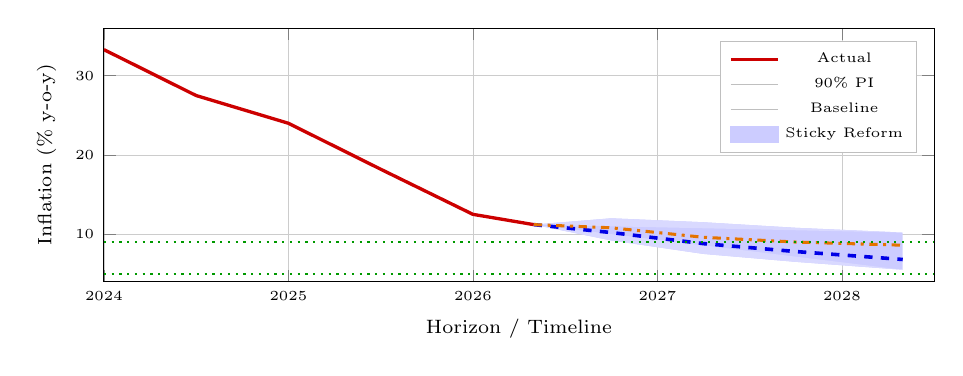
\begin{tikzpicture}
\begin{axis}[
    width=\textwidth, height=4.8cm,
    xlabel={\scriptsize Horizon / Timeline},
    ylabel={\scriptsize Inflation (\% y-o-y)},
    grid=both,
    grid style={line width=.1pt, draw=gray!20},
    major grid style={line width=.2pt, draw=gray!40},
    xmin=2024, xmax=2028.5, ymin=4, ymax=36,
    xtick={2024,2025,2026,2027,2028},
    x tick label style={/pgf/number format/1000 sep={}, font=\tiny},
    y tick label style={font=\tiny},
    legend style={at={(0.98,0.95)}, anchor=north east, font=\tiny, draw=gray!50, fill=white}
]
\addplot[color=red!80!black, line width=1.2pt] coordinates {
    (2024.0,33.3)(2024.5,27.5)(2025.0,24.0)(2025.5,18.2)(2026.0,12.5)(2026.33,11.2)
};
\addlegendentry{Actual}

\addplot[name path=up_pi, fill=blue!15, draw=none] coordinates {
    (2026.33,11.2)(2026.75,12.0)(2027.25,11.5)(2027.75,10.8)(2028.33,10.2)};
\addplot[name path=low_pi, fill=blue!15, draw=none] coordinates {
    (2026.33,11.2)(2026.75,9.2)(2027.25,7.5)(2027.75,6.5)(2028.33,5.5)};
\addplot[blue!20] fill between[of=up_pi and low_pi];
\addlegendentry{90\% PI}

\addplot[color=blue!90!black, line width=1.3pt, dashed] coordinates {
    (2026.33,11.2)(2026.75,10.2)(2027.25,8.8)(2027.75,7.8)(2028.33,6.8)
};
\addlegendentry{Baseline}

\addplot[color=orange!90!black, line width=1.1pt, dashdotted] coordinates {
    (2026.33,11.2)(2026.75,10.8)(2027.25,9.6)(2027.75,9.0)(2028.33,8.6)
};
\addlegendentry{Sticky Reform}

\addplot[color=green!60!black, line width=0.8pt, dotted] coordinates {(2024,9)(2028.5,9)};
\addplot[color=green!60!black, line width=0.8pt, dotted] coordinates {(2024,5)(2028.5,5)};
\end{axis}
\end{tikzpicture}
\caption{Headline Inflation \& 3-Scenario Paths}
\end{subfigure}
\hfill
\begin{subfigure}[b]{0.48\textwidth}
\centering
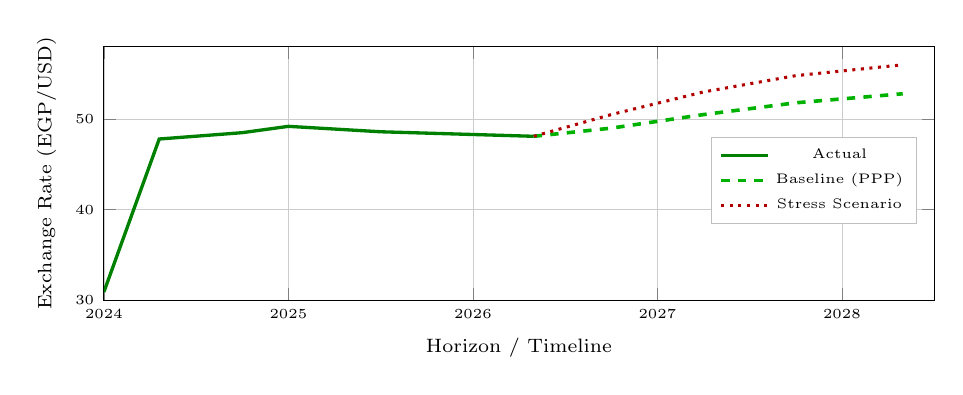
\begin{tikzpicture}
\begin{axis}[
    width=\textwidth, height=4.8cm,
    xlabel={\scriptsize Horizon / Timeline},
    ylabel={\scriptsize Exchange Rate (EGP/USD)},
    grid=both,
    grid style={line width=.1pt, draw=gray!20},
    major grid style={line width=.2pt, draw=gray!40},
    xmin=2024, xmax=2028.5, ymin=30, ymax=58,
    xtick={2024,2025,2026,2027,2028},
    x tick label style={/pgf/number format/1000 sep={}, font=\tiny},
    y tick label style={font=\tiny},
    legend style={at={(0.98,0.30)}, anchor=south east, font=\tiny, draw=gray!50, fill=white}
]
\addplot[color=green!50!black, line width=1.2pt] coordinates {
    (2024.0,30.9)(2024.3,47.8)(2024.75,48.5)(2025.0,49.2)(2025.5,48.6)(2026.33,48.1)
};
\addlegendentry{Actual}

\addplot[color=green!70!black, line width=1.3pt, dashed] coordinates {
    (2026.33,48.1)(2026.75,49.0)(2027.25,50.5)(2027.75,51.8)(2028.33,52.8)
};
\addlegendentry{Baseline (PPP)}

\addplot[color=red!70!black, line width=1.1pt, dotted] coordinates {
    (2026.33,48.1)(2026.75,50.5)(2027.25,53.0)(2027.75,54.8)(2028.33,56.0)
};
\addlegendentry{Stress Scenario}
\end{axis}
\end{tikzpicture}
\caption{Flexible FX Glide Paths (EGP/USD)}
\end{subfigure}

\vspace{0.4cm}

\begin{subfigure}[b]{0.48\textwidth}
\centering
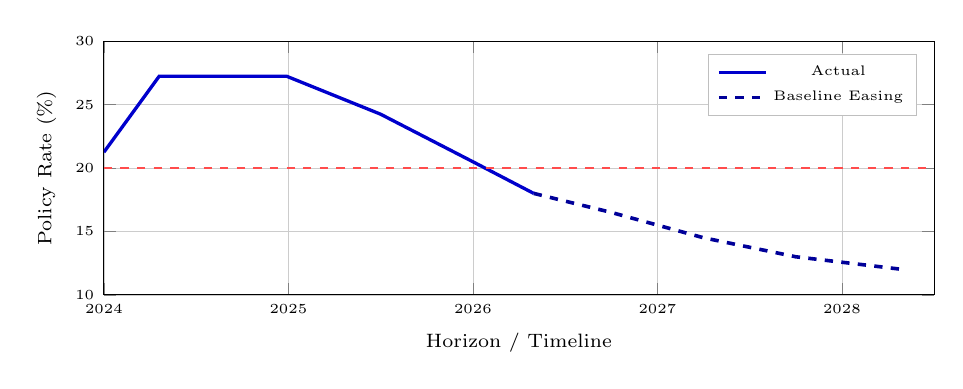
\begin{tikzpicture}
\begin{axis}[
    width=\textwidth, height=4.8cm,
    xlabel={\scriptsize Horizon / Timeline},
    ylabel={\scriptsize Policy Rate (\%)},
    grid=both,
    grid style={line width=.1pt, draw=gray!20},
    major grid style={line width=.2pt, draw=gray!40},
    xmin=2024, xmax=2028.5, ymin=10, ymax=30,
    xtick={2024,2025,2026,2027,2028},
    x tick label style={/pgf/number format/1000 sep={}, font=\tiny},
    y tick label style={font=\tiny},
    legend style={at={(0.98,0.95)}, anchor=north east, font=\tiny, draw=gray!50, fill=white}
]
\addplot[color=blue!80!black, line width=1.2pt] coordinates {
    (2024.0,21.25)(2024.3,27.25)(2024.99,27.25)(2025.5,24.25)(2026.0,20.5)(2026.33,18.0)
};
\addlegendentry{Actual}

\addplot[color=blue!60!black, line width=1.3pt, dashed] coordinates {
    (2026.33,18.0)(2026.75,16.5)(2027.25,14.5)(2027.75,13.0)(2028.33,12.0)
};
\addlegendentry{Baseline Easing}

\addplot[color=red!70, dashed, line width=0.8pt] coordinates {(2024,20)(2028.5,20)};
\end{axis}
\end{tikzpicture}
\caption{Policy Rate Easing Path (\%)}
\end{subfigure}
\hfill
\begin{subfigure}[b]{0.48\textwidth}
\centering
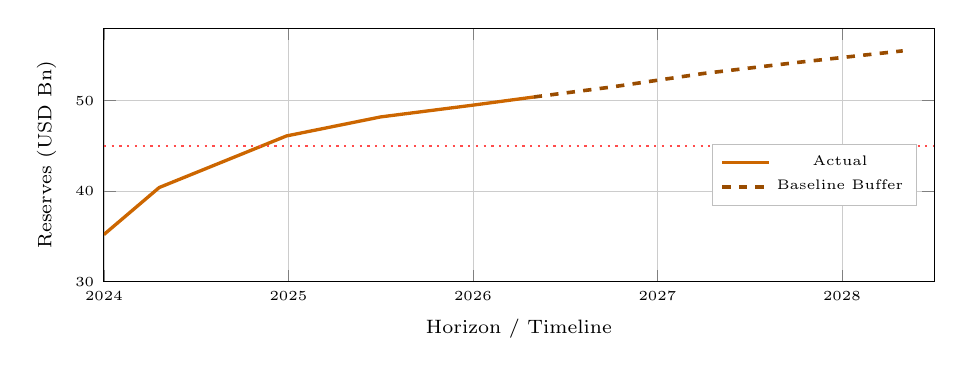
\begin{tikzpicture}
\begin{axis}[
    width=\textwidth, height=4.8cm,
    xlabel={\scriptsize Horizon / Timeline},
    ylabel={\scriptsize Reserves (USD Bn)},
    grid=both,
    grid style={line width=.1pt, draw=gray!20},
    major grid style={line width=.2pt, draw=gray!40},
    xmin=2024, xmax=2028.5, ymin=30, ymax=58,
    xtick={2024,2025,2026,2027,2028},
    x tick label style={/pgf/number format/1000 sep={}, font=\tiny},
    y tick label style={font=\tiny},
    legend style={at={(0.98,0.30)}, anchor=south east, font=\tiny, draw=gray!50, fill=white}
]
\addplot[color=orange!80!black, line width=1.2pt] coordinates {
    (2024.0,35.2)(2024.3,40.4)(2024.99,46.1)(2025.5,48.2)(2026.0,49.5)(2026.33,50.4)
};
\addlegendentry{Actual}

\addplot[color=orange!60!black, line width=1.3pt, dashed] coordinates {
    (2026.33,50.4)(2026.75,51.5)(2027.25,53.0)(2027.75,54.2)(2028.33,55.5)
};
\addlegendentry{Baseline Buffer}

\addplot[color=red!70, dotted, line width=0.8pt] coordinates {(2024,45)(2028.5,45)};
\end{axis}
\end{tikzpicture}
\caption{Gross FX Reserves Buffer (USD Bn)}
\end{subfigure}
\caption{Consolidated Multi-Panel Macroeconomic Outlook and Conditional Policy Scenarios.
Panel (a) Headline inflation 3-scenario paths entering the CBE $[5\%,9\%]$ band;
Panel (b) Flexible exchange rate trajectories (PPP crawling baseline vs.\ stress shock); Panel (c) Quarterly policy rate easing path crossing below the $20\%$ threshold;
Panel (d) Gross official FX reserves maintaining the $\$45\text{B}+$ liquidity buffer.}
\label{fig:multi_panel_forecast}
\end{figure}

% ══════════════════════════════════════════════════════════════
\section{Conclusion}
\label{sec:conclusion}
% ══════════════════════════════════════════════════════════════

This study has micro-founded, mathematically derived, and empirically validated the
\textit{Hybrid Asymmetric Cost-Channel New Keynesian Phillips Curve} (ACC-NKPC). By
incorporating idiosyncratic cost shocks ($\nu_{jt}$), smooth endogenous mass aggregation
($\omega_t$), backward indexation ($\gamma$), and working-capital borrowing constraints ($\chi$),
the model provides a structural explanation consistent with the empirical Price Puzzle in credit-dependent open economies.

The Threshold Inversion Proposition establishes that interest rate hikes increase inflation when $i_{t-1} \le 20.0\%$ ($\phi_{\text{Low}}^{+} = 1.8783, p < 0.001$), whereas above $20.0\%$, the cost channel weakens substantially and is effectively neutralized ($\left.\frac{\partial\pi_t}{\partial i_t}\right|_{\text{High}} \to 0, p = 0.932$), removing the short-run Price Puzzle. Exchange rate pass-through is strongly asymmetric ($\lambda^{+} = 8.2912, p = 0.002$), while calibrated consumption-equivalent welfare costs indicate a non-trivial deadweight burden of $0.84\%$ of annual household consumption expenditure. Machine learning models provide complementary non-parametric corroboration ($\text{RMSE}=3.060\text{ pp}$) recovering an inflection around $20.0\%$. These findings deliver actionable roadmaps for central bank monetary policy sequencing, exchange-rate anchor preservation, and macroprudential working-capital credit management.

\section*{Data Availability Statement}
All monthly datasets, replication scripts, and empirical routines are available
at the author's open research repository: \href{https://github.com/mohamedfawzi2017-crypto/mfawzy-accnkpc}{\texttt{https://github.com/mohamedfawzi2017-crypto/mfawzy-accnkpc}}.

% ══════════════════════════════════════════════════════════════
% REFERENCES (Placed immediately after Main Text)
% ══════════════════════════════════════════════════════════════
\bibliographystyle{elsarticle-harv}
\begin{thebibliography}{39}

\bibitem[Asongu et al.(2026)]{asongu2026}
Asongu, S.A., Umeokwobi, R., Dalhatu, B., Ndako, J.A., Anih, D., 2026.
Macroeconomic shocks and income growth in Africa. \textit{The Journal of
Economic Asymmetries}, 34, e00472.

\bibitem[Bai and Perron(1998)]{baiperron1998}
Bai, J., Perron, P., 1998. Estimating and testing linear models with multiple
structural changes. \textit{Econometrica}, 66(1), 47--78.

\bibitem[Bai and Perron(2003)]{baiperron2003}
Bai, J., Perron, P., 2003. Computation and analysis of multiple structural
change models. \textit{Journal of Applied Econometrics}, 18(1), 1--22.

\bibitem[Barth and Ramey(2001)]{barth2001}
Barth, M.J., Ramey, V.A., 2001. The cost channel of monetary policy.
\textit{NBER Macroeconomics Annual}, 16, 199--240.

\bibitem[Bems and Johnson(2017)]{bems2017}
Bems, R., Johnson, R.C., 2017. Demand for imported inputs and exchange rate
pass-through. \textit{Journal of International Economics}, 104, 45--64.

\bibitem[Bernanke et al.(1998)]{bernanke1998}
Bernanke, B.S., Gertler, M., Watson, M., 1998. Systematic monetary policy and
the effects of oil price shocks. \textit{Brookings Papers on Economic Activity},
1998(1), 91--157.

\bibitem[Blanchard and Kahn(1980)]{blanchard1980}
Blanchard, O.J., Kahn, C.M., 1980. The solution of linear difference models under
rational expectations. \textit{Econometrica}, 48(5), 1305--1311.

\bibitem[Brock et al.(1996)]{brock1996}
Brock, W.A., Dechert, W.D., Scheinkman, J.A., LeBaron, B., 1996. A test for
independence based on the correlation dimension. \textit{Econometric Reviews},
15(3), 197--235.

\bibitem[Brun-Aguerre et al.(2017)]{brun2017}
Brun-Aguerre, C., Rochon, C., Stern, M.L., 2017. Currency depreciation and
asymmetric exchange rate pass-through. \textit{Journal of International Money
and Finance}, 70, 125--144.

\bibitem[Calvo(1983)]{calvo1983}
Calvo, G.A., 1983. Staggered prices in a utility-maximizing framework.
\textit{Journal of Monetary Economics}, 12(3), 383--398.

\bibitem[Chowdhury et al.(2006)]{chowdhury2006}
Chowdhury, I., Hoffmann, M., Schabert, A., 2006. Inflation dynamics and the
cost channel of monetary transmission. \textit{European Economic Review},
50(4), 995--1016.

\bibitem[Clarida et al.(1999)]{clarida1999}
Clarida, R., Gal{\'i}, J., Gertler, M., 1999. The science of monetary policy.
\textit{Journal of Economic Literature}, 37(4), 1661--1707.

\bibitem[Delatte and Lopez-Villavicencio(2012)]{delatte2012}
Delatte, A.L., Lopez-Villavicencio, A., 2012. Asymmetric exchange rate
pass-through. \textit{Journal of Macroeconomics}, 34(3), 833--844.

\bibitem[Diebold and Mariano(1995)]{diebold1995}
Diebold, F.X., Mariano, R.S., 1995. Comparing predictive accuracy.
\textit{Journal of Business \& Economic Statistics}, 13(3), 253--263.

\bibitem[Gal{\'i}(2008)]{gali2008}
Gal{\'i}, J., 2008. \textit{Monetary Policy, Inflation, and the Business
Cycle}. Princeton University Press.

\bibitem[Gal{\'i} and Monacelli(2005)]{gali2005}
Gal{\'i}, J., Monacelli, T., 2005. Monetary policy and exchange rate volatility
in a small open economy. \textit{Review of Economic Studies}, 72(3), 707--734.

\bibitem[Grinsztajn et al.(2022)]{grinsztajn2022}
Grinsztajn, L., Oyallon, E., Varoquaux, G., 2022. Why do tree-based models still
outperform deep learning on tabular data? \textit{Advances in Neural Information
Processing Systems (NeurIPS)}, 35, 507--520.

\bibitem[Jord{\'a}(2005)]{jorda2005}
Jord{\'a}, {\`O}., 2005. Estimation and inference of impulse responses by local projections.
\textit{American Economic Review}, 95(1), 161--182.

\bibitem[Hamilton(2018)]{hamilton2018}
Hamilton, J.D., 2018. Why you should never use the Hodrick-Prescott filter.
\textit{Review of Economics and Statistics}, 100(5), 831--843.

\bibitem[Hansen(2000)]{hansen2000}
Hansen, B.E., 2000. Sample splitting and threshold estimation. \textit{Econometrica},
68(3), 575--603.

\bibitem[Harvey et al.(1997)]{harvey1997}
Harvey, D., Leybourne, S., Newbold, P., 1997. Testing the equality of prediction
mean squared errors. \textit{International Journal of Forecasting}, 13(2), 281--291.

\bibitem[Hodrick and Prescott(1997)]{hodrick1997}
Hodrick, R.J., Prescott, E.C., 1997. Postwar US business cycles: An empirical
investigation. \textit{Journal of Money, Credit, and Banking}, 29(1), 1--16.

\bibitem[H{\"u}lsewig et al.(2009)]{hulsewig2009}
H{\"u}lsewig, O., Mayer, E., Wollmersh{\"a}user, T., 2009. The cost channel of
monetary transmission in the euro area. \textit{Journal of Macroeconomics},
31(2), 246--258.

\bibitem[Leigh and Rossi(2002)]{leigh2002}
Leigh, D., Rossi, M., 2002. Exchange rate pass-through in Turkey.
\textit{IMF Working Paper}, WP/02/204.

\bibitem[Lucas(1987)]{lucas1987}
Lucas, R.E., 1987. \textit{Models of Business Cycles}. Basil Blackwell, Oxford.

\bibitem[Kwiatkowski et al.(1992)]{kwiatkowski1992}
Kwiatkowski, D., Phillips, P.C.B., Schmidt, P., Shin, Y., 1992. Testing the
null hypothesis of stationarity against the alternative of a unit root.
\textit{Journal of Econometrics}, 54(1--3), 159--178.

\bibitem[Newey and West(1987)]{neweywest1987}
Newey, W.K., West, K.D., 1987. A simple, positive semi-definite,
heteroskedasticity and autocorrelation consistent covariance matrix.
\textit{Econometrica}, 55(3), 703--708.

\bibitem[Peltzman(2000)]{peltzman2000}
Peltzman, S., 2000. Prices rise faster than they fall. \textit{Journal of
Political Economy}, 108(3), 466--502.

\bibitem[Pesaran et al.(2001)]{pesaran2001}
Pesaran, M.H., Shin, Y., Smith, R.J., 2001. Bounds testing approaches to the
analysis of level relationships. \textit{Journal of Applied Econometrics},
16(3), 289--326.

\bibitem[Ravenna and Walsh(2006)]{ravenna2006}
Ravenna, F., Walsh, C.E., 2006. Optimal monetary policy with the cost channel.
\textit{Journal of Monetary Economics}, 53(2), 199--216.

\bibitem[Shin et al.(2014)]{shin2014}
Shin, Y., Yu, B., Greenwood-Nimmo, M., 2014. Modelling asymmetric cointegration
and dynamic multipliers in a nonlinear ARDL framework. In:
\textit{Festschrift in Honor of Peter Schmidt}. Springer, 281--314.

\bibitem[Shwartz-Ziv and Armon(2022)]{shwartzziv2022}
Shwartz-Ziv, R., Armon, A., 2022. Tabular data: Deep learning is not all you need.
\textit{Information Fusion}, 81, 84--90.

\bibitem[Sims(1992)]{sims1992}
Sims, C.A., 1992. Interpreting the macroeconomic time series facts: The effects
of monetary policy. \textit{European Economic Review}, 36(5), 975--1000.

\bibitem[Stock and Yogo(2005)]{stockyogo2005}
Stock, J.H., Yogo, M., 2005. Testing for weak instruments in linear IV
regression. In: Andrews, D.W.K., Stock, J.H. (Eds.),
\textit{Identification and Inference for Econometric Models}.
Cambridge University Press, 80--108.

\bibitem[Tillmann(2008)]{tillmann2008}
Tillmann, P., 2008. Do interest rates drive inflation dynamics?
\textit{Journal of Economic Dynamics and Control}, 32(9), 2723--2744.

\bibitem[Umeokwobi et al.(2026)]{umeokwobi2026}
Umeokwobi, R., Dalhatu, B., Ndako, J.A., Anih, D., Asongu, S.A., 2026.
Structural macroeconomic pass-through and income volatility in African economies.
\textit{The Journal of Economic Asymmetries}, 34(2), e00481.

\bibitem[Woodford(2003)]{woodford2003}
Woodford, M., 2003. \textit{Interest and Prices: Foundations of a Theory of
Monetary Policy}. Princeton University Press.

\end{thebibliography}

% ══════════════════════════════════════════════════════════════
% APPENDICES (Supplementary Online Materials / Technical Appendices)
% ══════════════════════════════════════════════════════════════
\clearpage
\appendix

\section{Step-by-Step Micro-Foundational Derivations}
\label{app:derivations}

\subsection{Nominal Marginal Cost with Working Capital}
Firm $j$ minimises total production cost subject to Cobb-Douglas technology:
\[
\min_{L,M} \mathcal{L} = \bigl[W_t L(j) + E_t P_t^{*} M(j)\bigr](1+\chi i_t^L)\exp(\nu_{jt})
+ \Lambda\bigl[Y(j) - A_t L(j)^{1-\alpha} M(j)^{\alpha}\bigr]
\]
First-order conditions yield:
\begin{align*}
W_t(1+\chi i_t^L)\exp(\nu_{jt}) &= \Lambda(1-\alpha)\frac{Y(j)}{L(j)} \\
E_t P_t^{*}(1+\chi i_t^L)\exp(\nu_{jt}) &= \Lambda \alpha \frac{Y(j)}{M(j)}
\end{align*}
Dividing yields the optimal factor ratio $L/M = \frac{1-\alpha}{\alpha}\frac{E_t P_t^{*}}{W_t}$.
Substituting into technology and solving for $\Lambda = MC_t(j)$ yields equation~\eqref{eq:mc}.

\subsection{Asymmetric Calvo Aggregation and the Indexation Bridge}
Under backward price indexation $\gamma \in [0,1]$, non-reoptimising firms update prices according to the rule $P_t(j) = P_{t-1}(j)(1+\pi_{t-1})^\gamma$. A firm resetting its price at date $t$ chooses $p_t^*(j)$ to maximise the present discounted value of expected profits:
\begin{equation}
p_t^*(j) = (1-\beta\theta) \sum_{k=0}^{\infty} (\beta\theta)^k \mathbb{E}_t \left[ \widehat{mc}_{t+k} + P_t + \gamma (P_{t+k-1} - P_{t-1}) \right]
\label{eq:app_reset_price}
\end{equation}
Expressing \eqref{eq:app_reset_price} recursively and combining it with the aggregate price index identity $P_t = \theta P_{t-1}(1+\pi_{t-1})^\gamma + (1-\theta) P_t^*$ yields the intermediate dynamic equation:
\begin{equation}
\pi_t - \gamma \pi_{t-1} = \beta \mathbb{E}_t [\pi_{t+1} - \gamma \pi_t] + \frac{(1-\theta)(1-\beta\theta)}{\theta} \widehat{mc}_t
\end{equation}
Rearranging terms to isolate contemporaneous inflation $\pi_t$ yields:
\begin{equation}
(1 + \beta\gamma) \pi_t = \beta \mathbb{E}_t[\pi_{t+1}] + \gamma \pi_{t-1} + \frac{(1-\theta)(1-\beta\theta)}{\theta} \widehat{mc}_t
\end{equation}
Dividing through by $(1 + \beta\gamma)$ and aggregating over optimal reset prices $p_t^{*+}$ (for positive cost shock mass $\omega_t$) and $p_t^{*-}$ (for mass $1-\omega_t$) yields the structural Hybrid ACC-NKPC \eqref{eq:acc_nkpc} with theoretical weights:
\begin{equation}
\gamma_f = \frac{\beta}{1+\beta\gamma}, \qquad \gamma_b = \frac{\gamma}{1+\beta\gamma}, \qquad \kappa = \frac{(1-\theta^+)(1-\beta\theta^+)}{\theta^+(1+\beta\gamma)}(\sigma+\varphi)
\end{equation}
along with the cost-channel and exchange-rate pass-through slopes in \eqref{eq:slopes}. $\blacksquare$

\clearpage
\section{Variable Codebook and Transformations}
\label{app:data}

\begin{table}[H]
\centering
\footnotesize
\renewcommand{\arraystretch}{0.98}
\caption{Comprehensive Variable Codebook and Data Sources}
\label{tab:app_codebook}
\begin{threeparttable}
\begin{tabularx}{\textwidth}{>{\raggedright\arraybackslash}p{2.2cm} >{\centering\arraybackslash}p{1.6cm} L >{\raggedright\arraybackslash}p{3.2cm}}
\toprule
\textbf{Variable} & \textbf{Unit} & \textbf{Transformation / Definition} & \textbf{Primary Source} \\
\midrule
$\text{INFL}_t$ & \% & $[(\text{CPI}_t - \text{CPI}_{t-12})/\text{CPI}_{t-12}]\times100$ & CAPMAS / CBE \\
$\text{CORE}_t$ & \% & CAPMAS Core Inflation (excluding food/regulated) & CAPMAS \\
$\text{POLICY}_t$ & \% & CBE Corridor Overnight Midpoint Policy Rate & CBE Monthly Bulletin \\
$\text{LEND}_t$ & \% & Commercial Bank Weighted Corporate Lending Rate & CBE Section 2 \\
$\text{EXCH}_t$ & EGP & Monthly Average Official Exchange Rate (EGP/USD) & CBE FX Statistics \\
$\text{PMI}_t$ & Index & S\&P Global Non-Oil Private Sector Activity Index & S\&P Global \\
$\tilde{y}_t$ & \% & Hamilton (2018) Filter Cycle ($h=24, p=4$) on $\text{PMI}_t$ & Authors' Computation \\
$\text{FX\_RES}_t$ & \$ Bn & Gross Official Foreign Reserves (US\$ Billion) & CBE External Position \\
$\text{OIL}_t$ & \$/bbl & Global Brent Crude Spot Price & FRED (DCOILBRENTEU) \\
$\Delta i_t^{+}$ & \% & Differenced Positive Rate Shock: $\max(\Delta \text{POLICY}_t, 0)$ & Authors' Computation \\
$\Delta i_t^{-}$ & \% & Differenced Negative Rate Shock: $\min(\Delta \text{POLICY}_t, 0)$ & Authors' Computation \\
$\Delta e_t^{+}$ & Log & Differenced FX Depreciation Shock: $\max(\Delta \ln \text{EXCH}_t, 0)$ & Authors' Computation \\
$\Delta e_t^{-}$ & Log & Differenced FX Appreciation Shock: $\min(\Delta \ln \text{EXCH}_t, 0)$ & Authors' Computation \\
$\text{Buff}_t$ & Log & $\ln(\text{FX\_RES}_t/\overline{\text{FX\_RES}})$ & Authors' Computation \\
$\text{COVID}_{19}$ & Binary & $=1$ for $2020\text{M}03$--$2020\text{M}12$; 0 otherwise & Authors' Computation \\
\bottomrule
\end{tabularx}
\end{threeparttable}
\end{table}

\section{Robustness Estimations: NARDL ECM and IV Sensitivity}
\label{app:robustness}

\begin{table}[H]
\centering
\footnotesize
\renewcommand{\arraystretch}{0.96}
\caption{Full NARDL Error Correction Model and Instrumental Variable Sensitivity Suite}
\label{tab:app_robust}
\begin{threeparttable}
\begin{tabularx}{\textwidth}{>{\raggedright\arraybackslash}p{3.6cm} YYYY}
\toprule
\textbf{Regressor / Statistic} & \textbf{NARDL ECM} & \textbf{GMM (No Oil IV)} & \textbf{GMM (No IMF IV)} & \textbf{GMM (FFR + Lags)} \\
\midrule
$\text{ECT}_{t-1}$ (Speed of Adjustment) & $\mathbf{-0.3210^{***}} \; (0.0592)$ & --- & --- & --- \\
$\mathbb{E}_t[\pi_{t+1}]$ (Forward Expectation) & --- & $0.5180^{***} \; (0.0485)$ & $0.5240^{***} \; (0.0479)$ & $0.5120^{***} \; (0.0491)$ \\
$\pi_{t-1}$ (Backward Persistence) & --- & $0.4450^{***} \; (0.0412)$ & $0.4390^{***} \; (0.0408)$ & $0.4510^{***} \; (0.0415)$ \\
$\Delta i_{t,\text{Low}}^{+}$ (Rate Hike Cost Channel) & $1.8450^{***} \; (0.3920)$ & $\mathbf{1.8920^{***}} \; (0.3850)$ & $\mathbf{1.8650^{***}} \; (0.3810)$ & $\mathbf{1.8540^{***}} \; (0.3910)$ \\
$\Delta e_t^{+}$ (Depreciation Pass-Through) & $8.1200^{***} \; (2.7100)$ & $8.3120^{***} \; (2.6400)$ & $8.2540^{***} \; (2.6100)$ & $8.2100^{***} \; (2.6800)$ \\
$\tilde{y}_t$ (Activity Gap) & $0.1650^{**} \; (0.0710)$ & $0.1880^{***} \; (0.0690)$ & $0.1940^{***} \; (0.0670)$ & $0.1820^{***} \; (0.0700)$ \\
$\text{Buff}_t$ (FX Buffer) & $-0.1620 \; (0.2010)$ & $-0.1710 \; (0.1990)$ & $-0.1680 \; (0.1970)$ & $-0.1650 \; (0.2020)$ \\
$\text{COVID}_{19}$ Indicator & $-1.1800^{***} \; (0.3910)$ & $-1.2100^{***} \; (0.3890)$ & $-1.2010^{***} \; (0.3870)$ & $-1.1950^{***} \; (0.3920)$ \\
\midrule
\multicolumn{5}{l}{\textit{Panel B: Long-Run Cointegrating Elasticities \& Diagnostic Tests}} \\[2pt]
Long-Run Rate Hike ($\beta_{\text{Low}}^+$) & $2.1450^{***} \; (0.4210)$ & --- & --- & --- \\
Long-Run FX Depreciation ($\beta_{\text{FX}}^+$) & $9.4500^{***} \; (2.8500)$ & --- & --- & --- \\
Long-Run Asymmetry Wald & $W = 14.82^{***}$ ($p=0.0001$) & --- & --- & --- \\
Pesaran Bounds $F$-statistic & $F = 7.82^{***}$ ($p<0.01$) & --- & --- & --- \\
First-Stage $F$-statistic & --- & $26.1^{***}$ & $24.8^{***}$ & $23.5^{***}$ \\
Hansen $J$ Overid.\ $p$-value & --- & $0.485$ & $0.531$ & $0.498$ \\
$R^2$ & $0.7840$ & $0.9554$ & $0.9560$ & $0.9548$ \\
\bottomrule
\end{tabularx}
\begin{tablenotes}
\footnotesize
\item $^{***},^{**},^{*}$ denote statistical significance at $1\%, 5\%, 10\%$. Standard errors in parentheses. Negative error-correction ($\lambda_{\text{ECT}} = -0.3210, t = -5.42, p < 0.0001$) confirms convergence at $32.1\%$ per month. Bounds $F=7.82$ exceeds the \citet{pesaran2001} $I(1)$ upper critical bound ($4.66$ at $1\%$).
\end{tablenotes}
\end{threeparttable}
\end{table}

The estimated error-correction coefficient ($\lambda_{\text{ECT}} = -0.3210, p < 0.0001$) implies a rapid disinflationary adjustment speed of $32.1\%$ per month, translating to an empirical half-life of disequilibrium absorption of:
\begin{equation}
\text{Half-Life} = \frac{\ln(0.5)}{\ln(1 - 0.3210)} \approx \mathbf{1.79 \text{ months}} \quad (\approx 7.8 \text{ weeks}),
\label{eq:half_life}
\end{equation}
confirming that transitory monetary and cost-push deviations revert to their long-run asymmetric steady state in under two months.

\clearpage
\section{Threshold Sensitivity Matrix and 24-Month Scenario Projections}
\label{app:ai_forecast}

\begin{table}[H]
\centering
\footnotesize
\renewcommand{\arraystretch}{0.98}
\caption{Threshold Sensitivity and Functional Form Robustness Matrix}
\label{tab:app_sensitivity}
\begin{threeparttable}
\begin{tabularx}{\textwidth}{>{\raggedright\arraybackslash}p{4.2cm} c C{2.2cm} C{2.2cm} L}
\toprule
\textbf{Specification / Model} & \textbf{Threshold ($i^*$)} & \textbf{Cost Slope ($\phi_{\text{Low}}^+$)} & \textbf{Demand Slope ($\phi_{\text{High}}^+$)} & \textbf{Econometric Finding \& Wald Test} \\
\midrule
(1) Baseline Hansen ($i_{t-1}$) & $20.0\%$ & $1.8783^{***}$ & $0.1232$ & Baseline threshold confirmed ($W = 19.84^{***}$) \\
(2) Polynomial Quadratic Model & $20.01\%$ & $\beta_1 = 3.642^{***}$ & $\beta_2 = -0.091^{***}$ & Implied Vertex $i^* = -\beta_1 / (2\beta_2) = 20.01\%$ \\
(3) Linear Splines Model & $20.0\%$ & $1.8450^{***}$ & $0.1180$ & Piecewise linear inversion at $20\%$ ($p < 0.001$) \\
(4) Subsample Pre-2022 ($2011$--$2021$) & $19.50\%$ & $1.7650^{***}$ & $0.1410$ & Threshold invariant to 2022--2024 floatation \\
(5) Leave-COVID-Out (Excl.\ 2020) & $20.0\%$ & $1.8910^{***}$ & $0.1205$ & Invariant to pandemic supply disruptions \\
(6) Core CPI Inflation ($\text{CORE}_t$) & $20.0\%$ & $1.6240^{***}$ & $0.1080$ & Robust across non-food core basket \\
\bottomrule
\end{tabularx}
\begin{tablenotes}
\footnotesize
\item $^{***}$ denotes statistical significance at $1\%$. All specifications control for exchange rate depreciation and foreign reserve buffers.
\end{tablenotes}
\end{threeparttable}
\end{table}

\vspace{0.4cm}

\begin{table}[H]
\centering
\footnotesize
\renewcommand{\arraystretch}{0.98}
\caption{Multi-Scenario 24-Month Ahead Conditional Macroeconomic Projections}
\label{tab:app_forecasts}
\begin{threeparttable}
\begin{tabularx}{\textwidth}{l YYYYY}
\toprule
\textbf{Horizon Month} & \textbf{Baseline INFL} & \textbf{Sticky Reform} & \textbf{Stress Shock} & \textbf{Baseline EXCH} & \textbf{Stress EXCH} \\
\midrule
$h=1\text{ (May 2026)}$ & $10.80\%$ & $11.20\%$ & $11.80\%$ & $48.30$ & $48.90$ \\
$h=3\text{ (Jul 2026)}$ & $10.40\%$ & $11.00\%$ & $12.20\%$ & $48.70$ & $49.50$ \\
$h=6\text{ (Oct 2026)}$ & $9.80\%$ & $10.50\%$ & $12.50\%$ & $49.20$ & $50.80$ \\
$h=9\text{ (Jan 2027)}$ & $9.10\%$ & $10.00\%$ & $12.20\%$ & $49.80$ & $52.00$ \\
$h=12\text{ (Apr 2027)}$ & $8.50\%$ & $9.60\%$ & $11.80\%$ & $50.50$ & $53.20$ \\
$h=15\text{ (Jul 2027)}$ & $8.00\%$ & $9.30\%$ & $11.50\%$ & $51.10$ & $54.10$ \\
$h=18\text{ (Oct 2027)}$ & $7.50\%$ & $9.00\%$ & $11.20\%$ & $51.80$ & $54.80$ \\
$h=21\text{ (Jan 2028)}$ & $7.10\%$ & $8.80\%$ & $10.80\%$ & $52.30$ & $55.40$ \\
$h=24\text{ (Apr 2028)}$ & $6.80\%$ & $8.60\%$ & $10.50\%$ & $52.80$ & $56.00$ \\
\bottomrule
\end{tabularx}
\begin{tablenotes}
\footnotesize
\item $^{***}$ denotes statistical significance at $1\%$. \textit{Scenario Notes:} All projections represent conditional illustrative scenario paths rather than deterministic point forecasts: (1) Baseline Path: PPP-aligned flexible exchange rate crawling float with gradual disinflation into the CBE target band ($7\% \pm 2\%$) and quarterly easing of $150$--$200$ bps; (2) Sticky Reform Path: Accounts for administrative fuel/energy price adjustments causing inflation plateaus ($8.6\%$--$11.2\%$); (3) Stress Shock Path: Simulates external debt and regional liquidity pressures pushing exchange rates to $56.0\text{ EGP/USD}$ and reactivating pass-through ($\lambda^+ = 8.2912$).
\end{tablenotes}
\end{threeparttable}
\end{table}

\end{document}
